
%% %%
%% %% INTRO
%% %%

\slide{ Status and Todo list }
{
Wmunu integrated, single- and double-differential measurements largely finished.\\
Last two months: concentrated effort to understand A vs C-side discrepancies. \\

What remains to be done:
\iteb
\item Single and Double-differential asymmetries
\iteb
\item Code ready to make asymmetries from non-extrapolated measurements
\item Wild swings in theory uncertainty - waiting for increased sample statistics
\itee
\item Check if additional pileup uncertainty is needed (e.g., effect on QCD fits)
\item Finalize treatment of systematic ``smoothing'' (if needed after sample updates)
\itee
}

\slide{ Recent updates }
{
CombinationInputs v8 (wmunu version: v6):
\iteb
\item Switched from mu18\_MG (buggy) to mu18 trigger
\item Increased number of MC toys (for SFs) from 100 to 1000
\itee
CombinationInputs vX (wmunu version v7) - \red{not uploaded yet}
\iteb
\item Fixed a bug that treated uncorrelated portion of QCD uncertainty as correlated
\item Added full difference between MET and W\_mT fits to QCD systematics
\item Wpt systematic updated to sum-in-quadrature of Sherpa14MC11 and PowhegPythia8MC11
\itee
}

\slide{ A vs C-side problem }
{
  We discovered a \red{serious problem} with the \red{mu18MG triggers on the C-side}. This problem \red{cannot be corrected with Z tag-and-probe} because of the (yet unknown) bug with AOD and D3PD-based trigger matching. 
}

\slide{ BEFORE: A/C ratio }
{
\colb[T]
\column{.5\textwidth}
\centering
\small{ $W^{+}$}
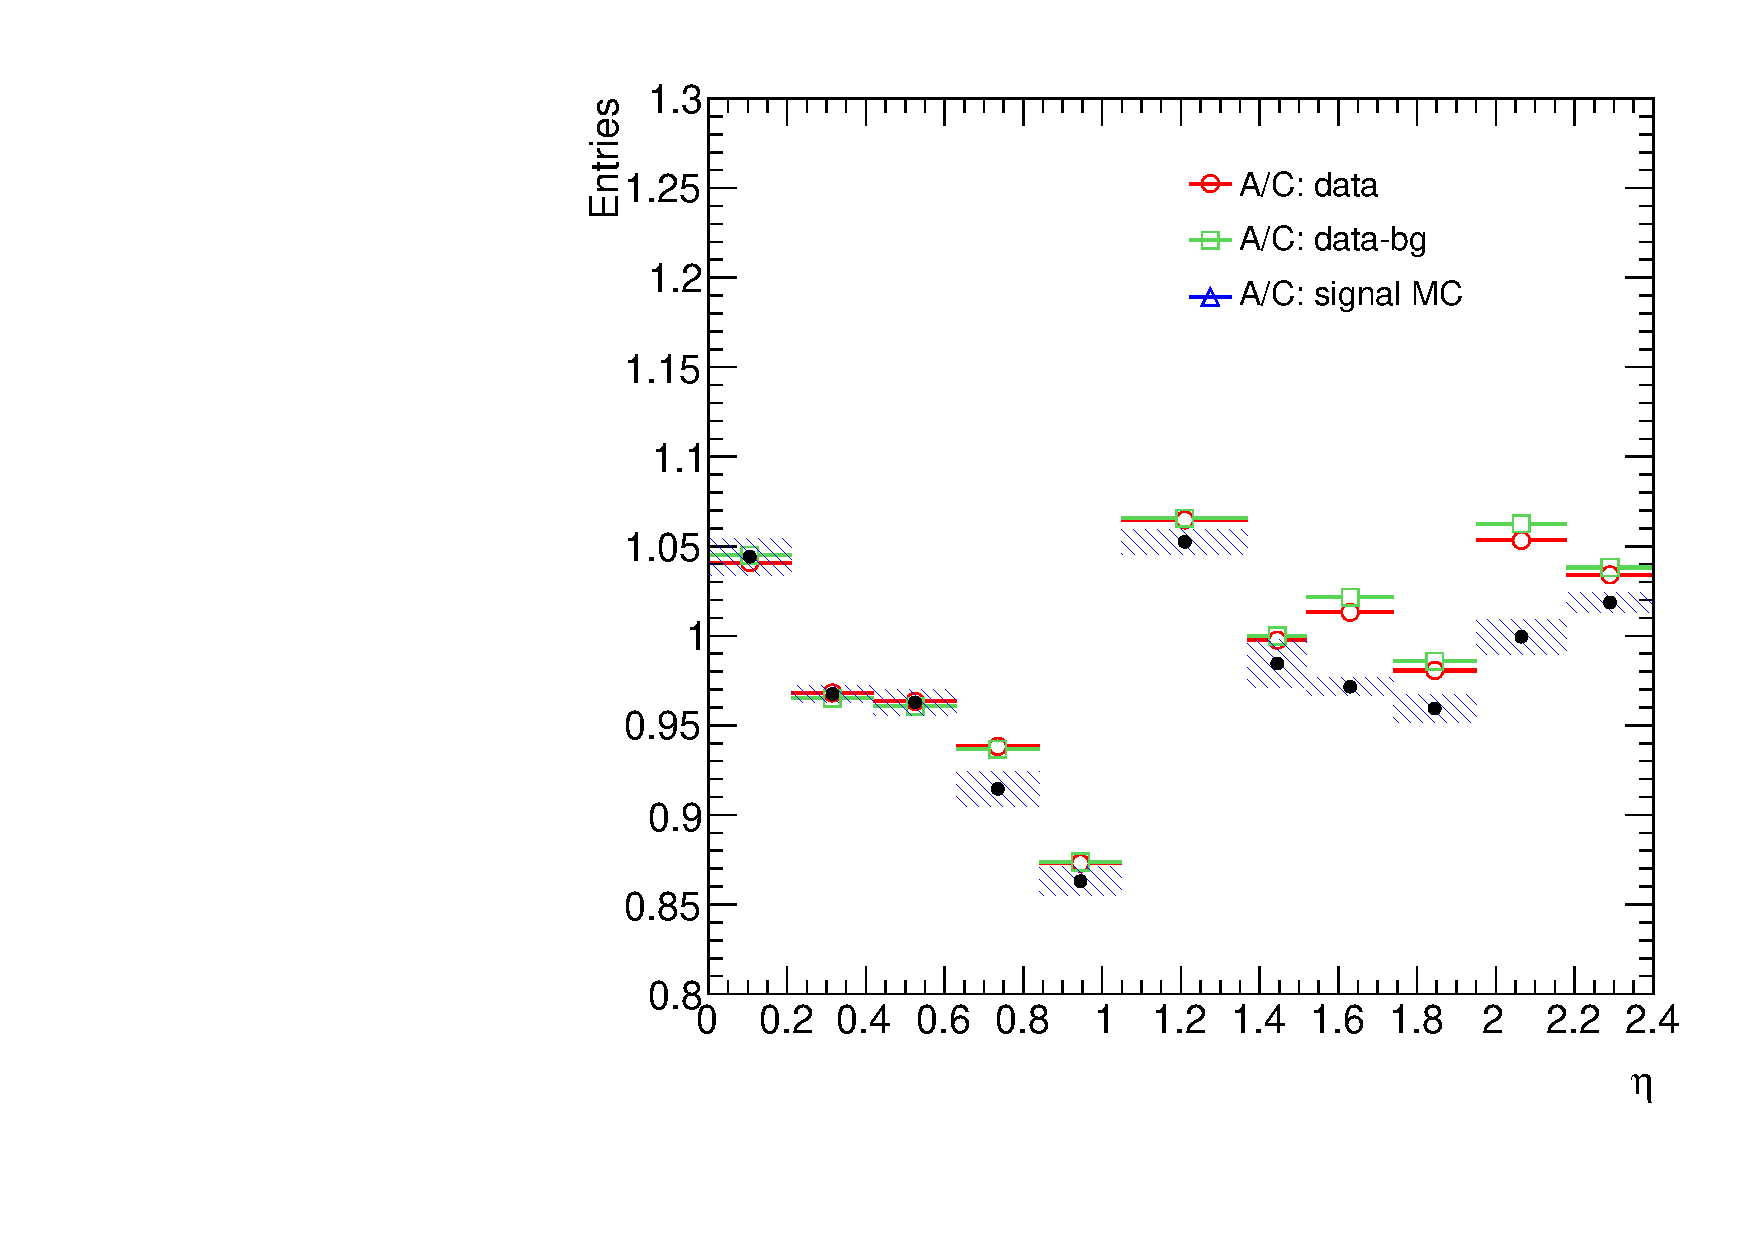
\includegraphics[width=1.0\textwidth]{dates/20130403/figures/old/ACSIDE/W_NOM_Q0_stack_d3_eta_lpt_met_y_2__1_z_0__1_POS}
\column{.5\textwidth}
\centering
\small{ $W^{-}$}
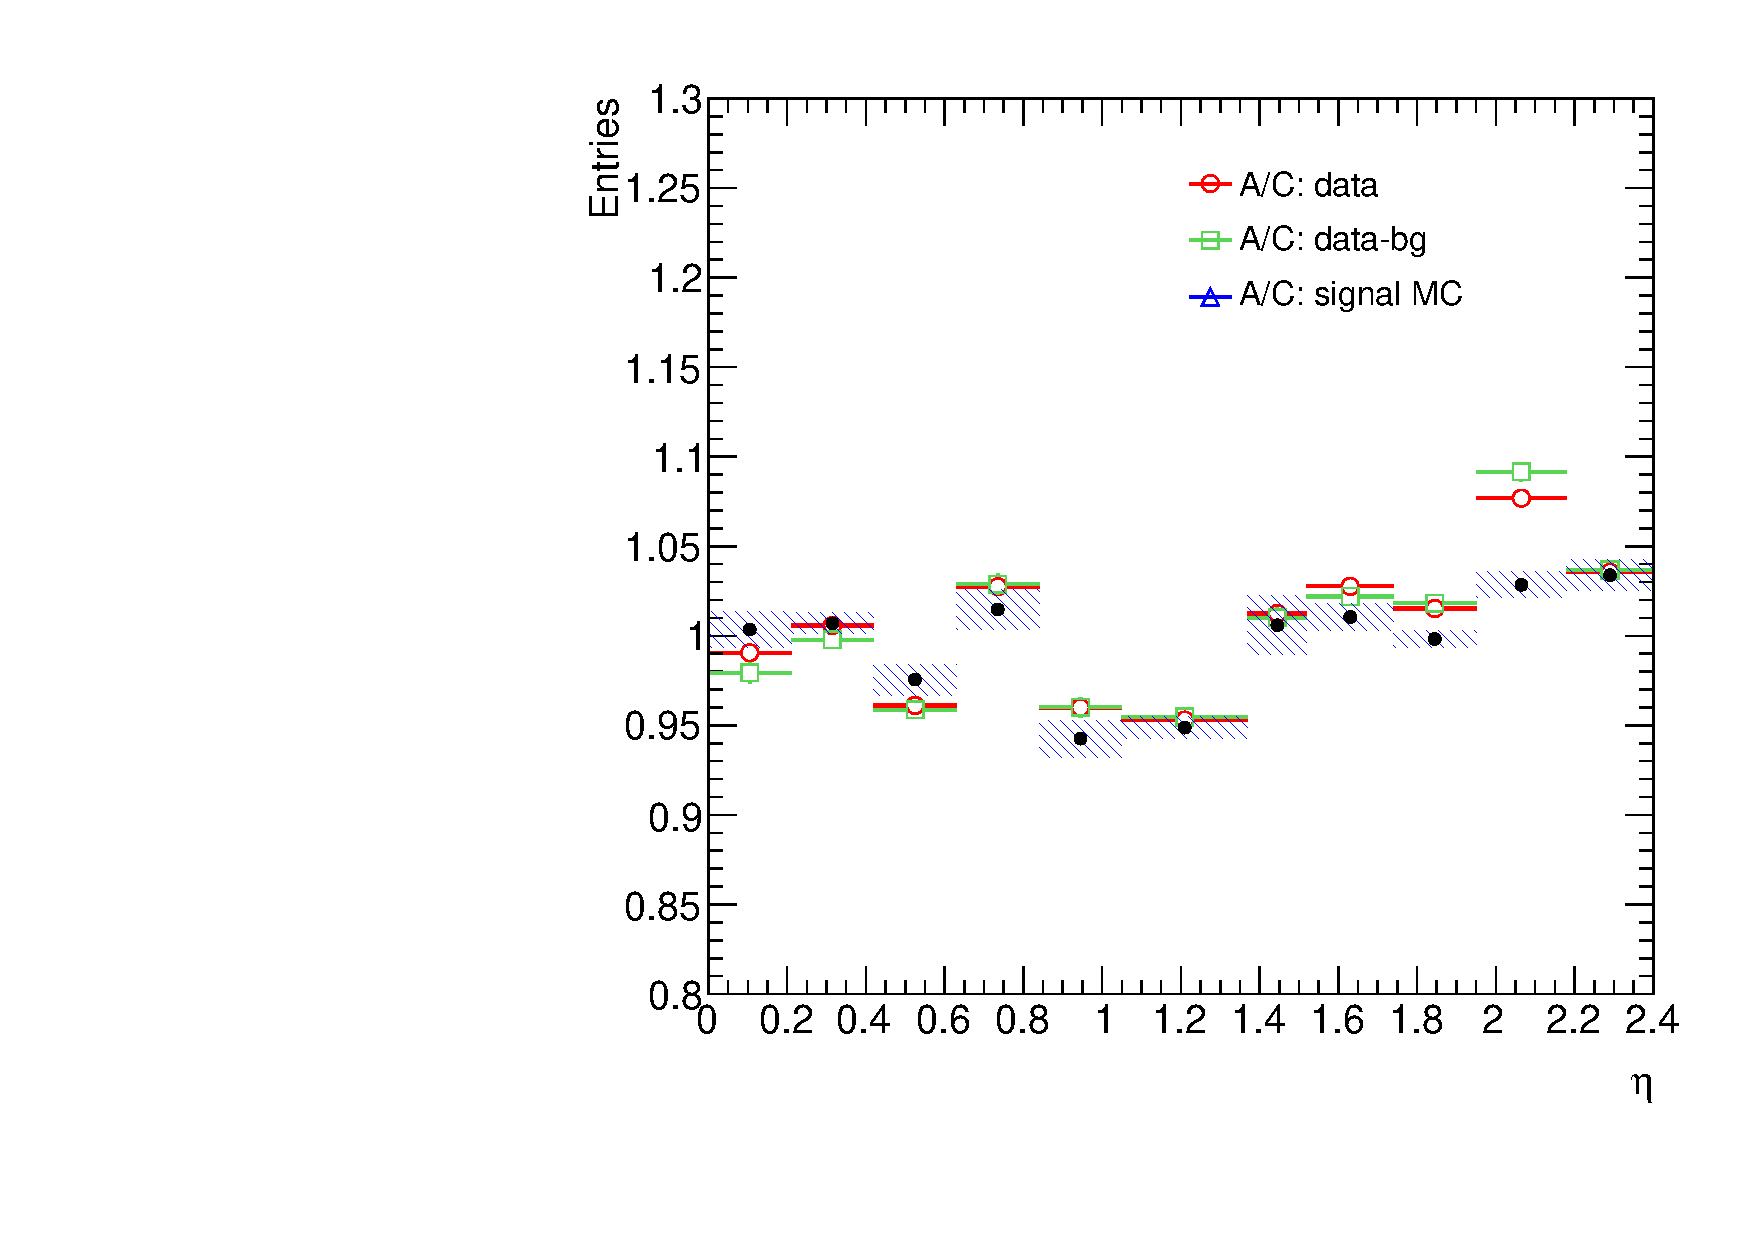
\includegraphics[width=1.0\textwidth]{dates/20130403/figures/old/ACSIDE/W_NOM_Q0_stack_d3_eta_lpt_met_y_2__1_z_0__1_NEG}
\cole
}

\slide{ LATEST: A/C ratio }
{
\colb[T]
\column{.5\textwidth}
\centering
\small{ $W^{+}$}
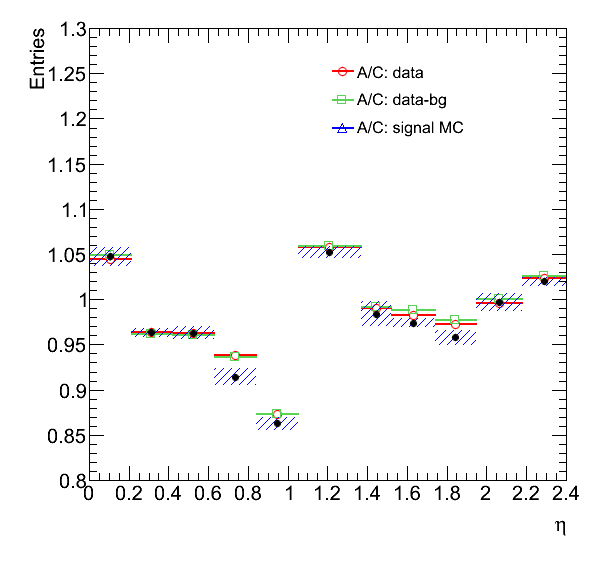
\includegraphics[width=1.0\textwidth]{dates/20130403/figures/new/ACSIDE/W_NOM_Q0_stack_d3_eta_lpt_met_y_2__1_z_0__1_POS}
\column{.5\textwidth}
\centering
\small{ $W^{-}$}
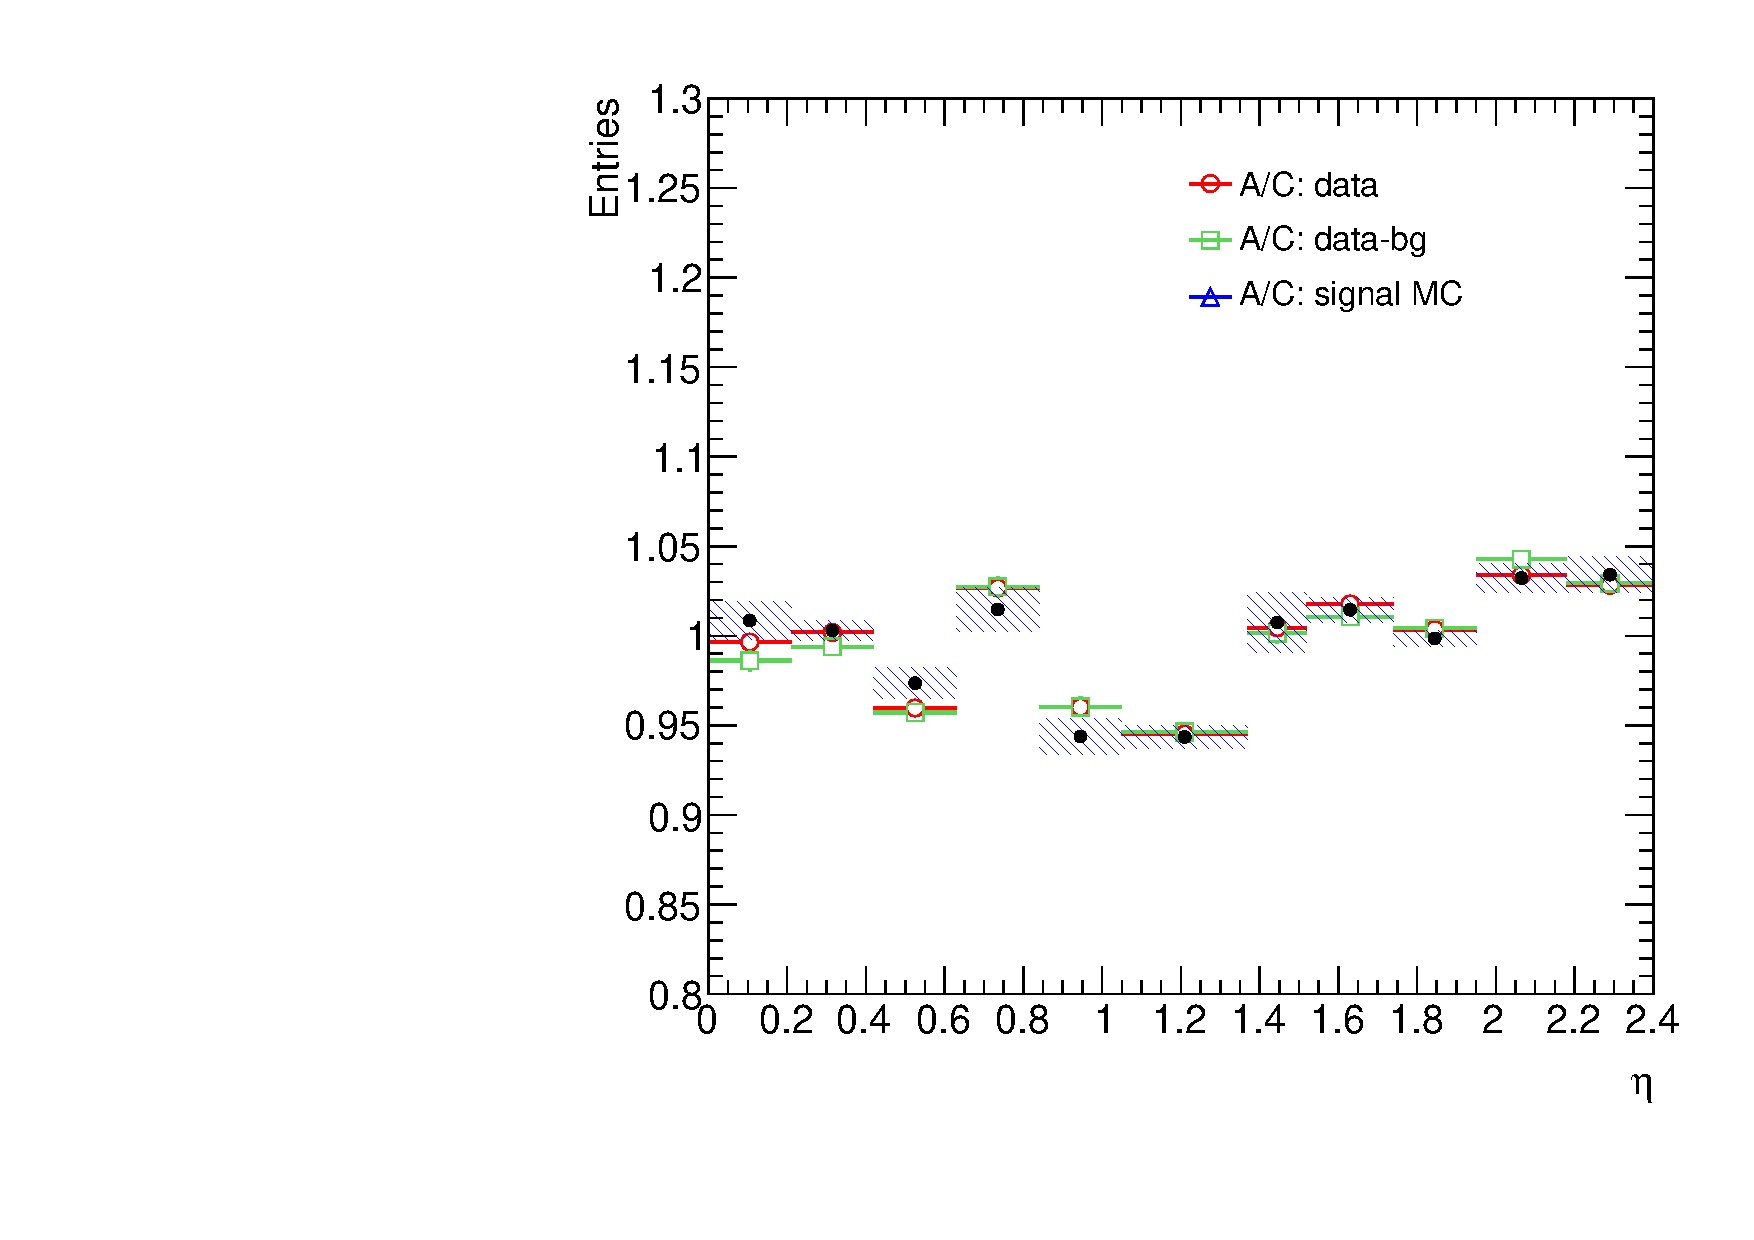
\includegraphics[width=1.0\textwidth]{dates/20130403/figures/new/ACSIDE/W_NOM_Q0_stack_d3_eta_lpt_met_y_2__1_z_0__1_NEG}
\cole
}

\slide{ mu18 vs mu18MG  } {
 Below, 2D eta-phi plots for full W selection, where:
 \iteb
 \item mu18MG trigger fails, but mu18 succeeds
 \itee
}

\slide{ mu18MG vs mu18: mu18 succeeds  } {
\colb[T]
\column{.5\textwidth}
$\mu^+$: Period D
\centering
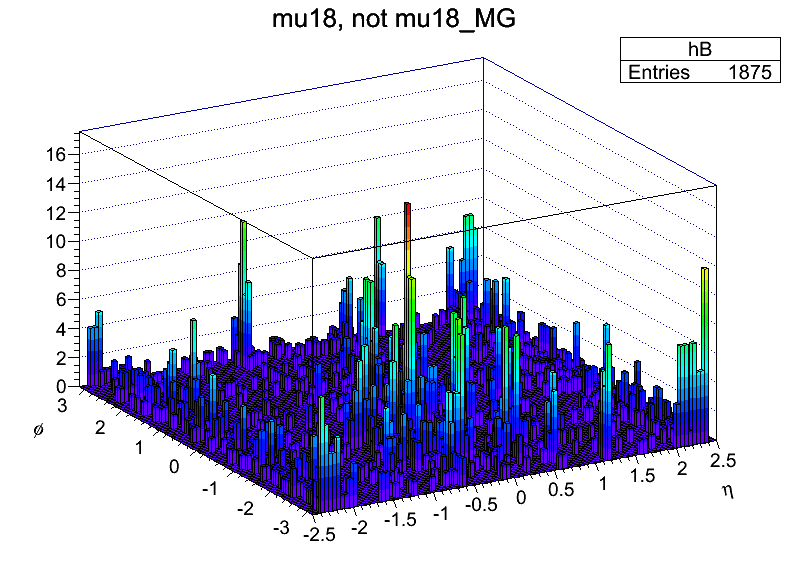
\includegraphics[width=0.95\textwidth]{dates/20130306/figures/mu18/dump_MG_dataD_w_POS.dat__MUID_NOT_MG.png}
\column{.5\textwidth}
$\mu^-$: Period D
\centering
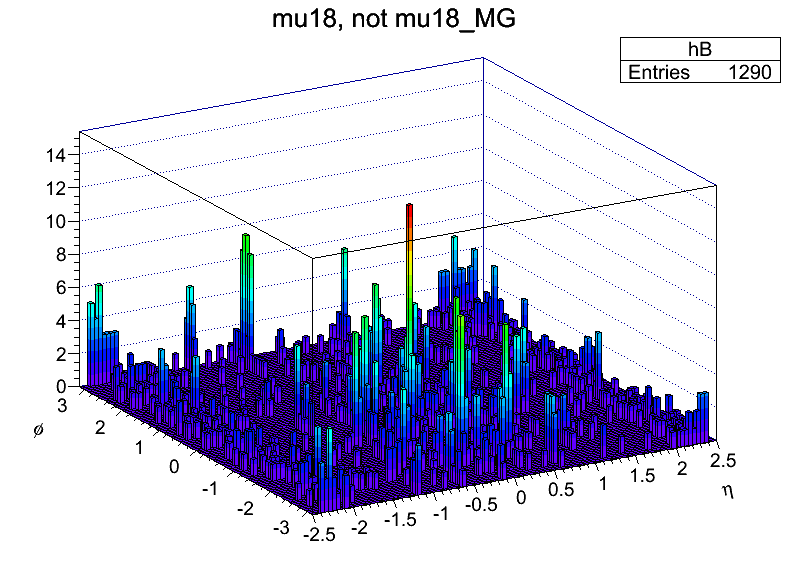
\includegraphics[width=0.95\textwidth]{dates/20130306/figures/mu18/dump_MG_dataD_w_NEG.dat__MUID_NOT_MG.png}
\cole
}
\slide{ mu18MG vs mu18: mu18MG succeeds  } {
\colb[T]
\column{.5\textwidth}
$\mu^+$: Period L
\centering
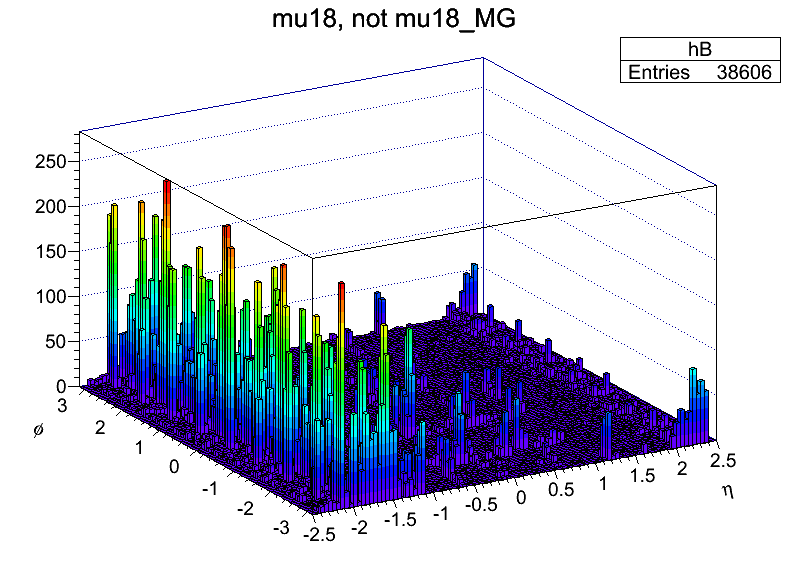
\includegraphics[width=0.95\textwidth]{dates/20130306/figures/mu18/dump_MG_dataL_w_POS.dat__MUID_NOT_MG.png}
\column{.5\textwidth}
$\mu^-$: Period L
\centering
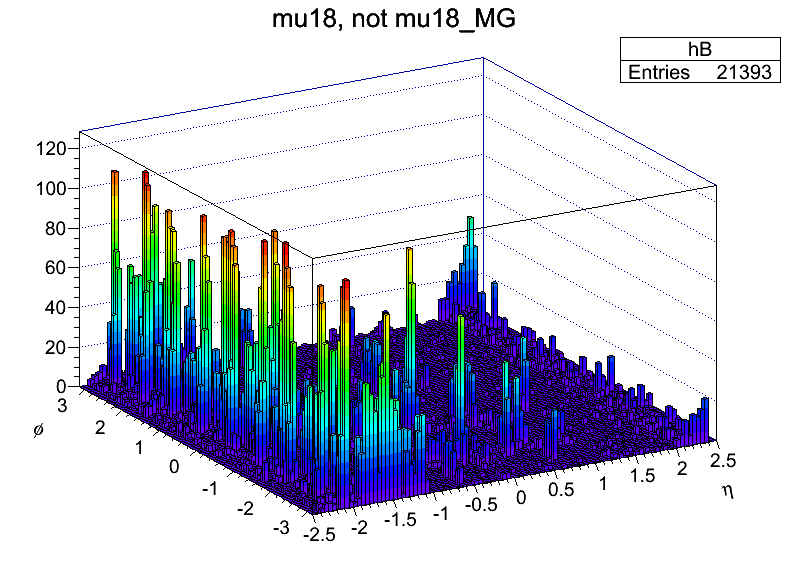
\includegraphics[width=0.95\textwidth]{dates/20130306/figures/mu18/dump_MG_dataL_w_NEG.dat__MUID_NOT_MG.png}
\cole
}
\slide{ mu18 vs mu18MG  } {
  Conclusions: \\
  Remember that these plots do not rely on trigger matching - we simply use W selection with 1 muon, which HAD to trigger.
  We see that \red{something happened to the MG trigger on the C-side in later data periods}. The mu18 trigger is not affected.
}

\slide{ Inside one of the ``bad'' measurement bins  }
{
MG triggers exhibit strange narrow-eta efficiency dips, which are not seen in Z events and thus not caught by tag-and-probe.
}

\slide{ $\mu^{+}$: bin 10 ($1.95<\eta<2.18$) } {
\colb[T]
\column{.5\textwidth}
C-side $\mu^{+}$ (top: W; bottom: Z)
\centering
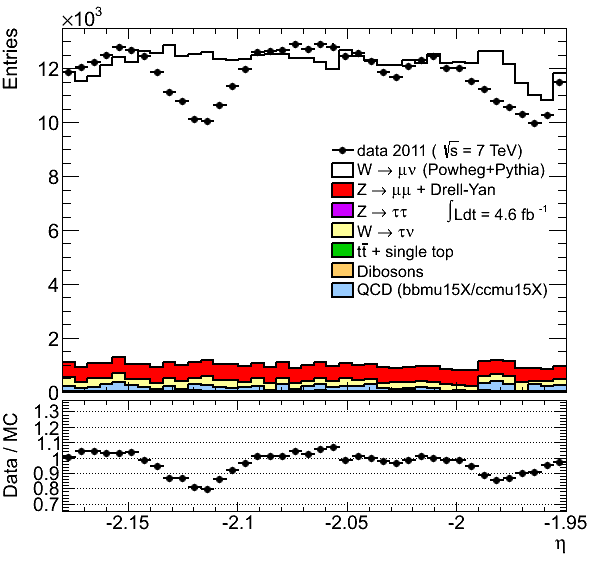
\includegraphics[width=0.66\textwidth]{dates/20130306/figures/both/W_10_C_stack_l_eta_POS} \\
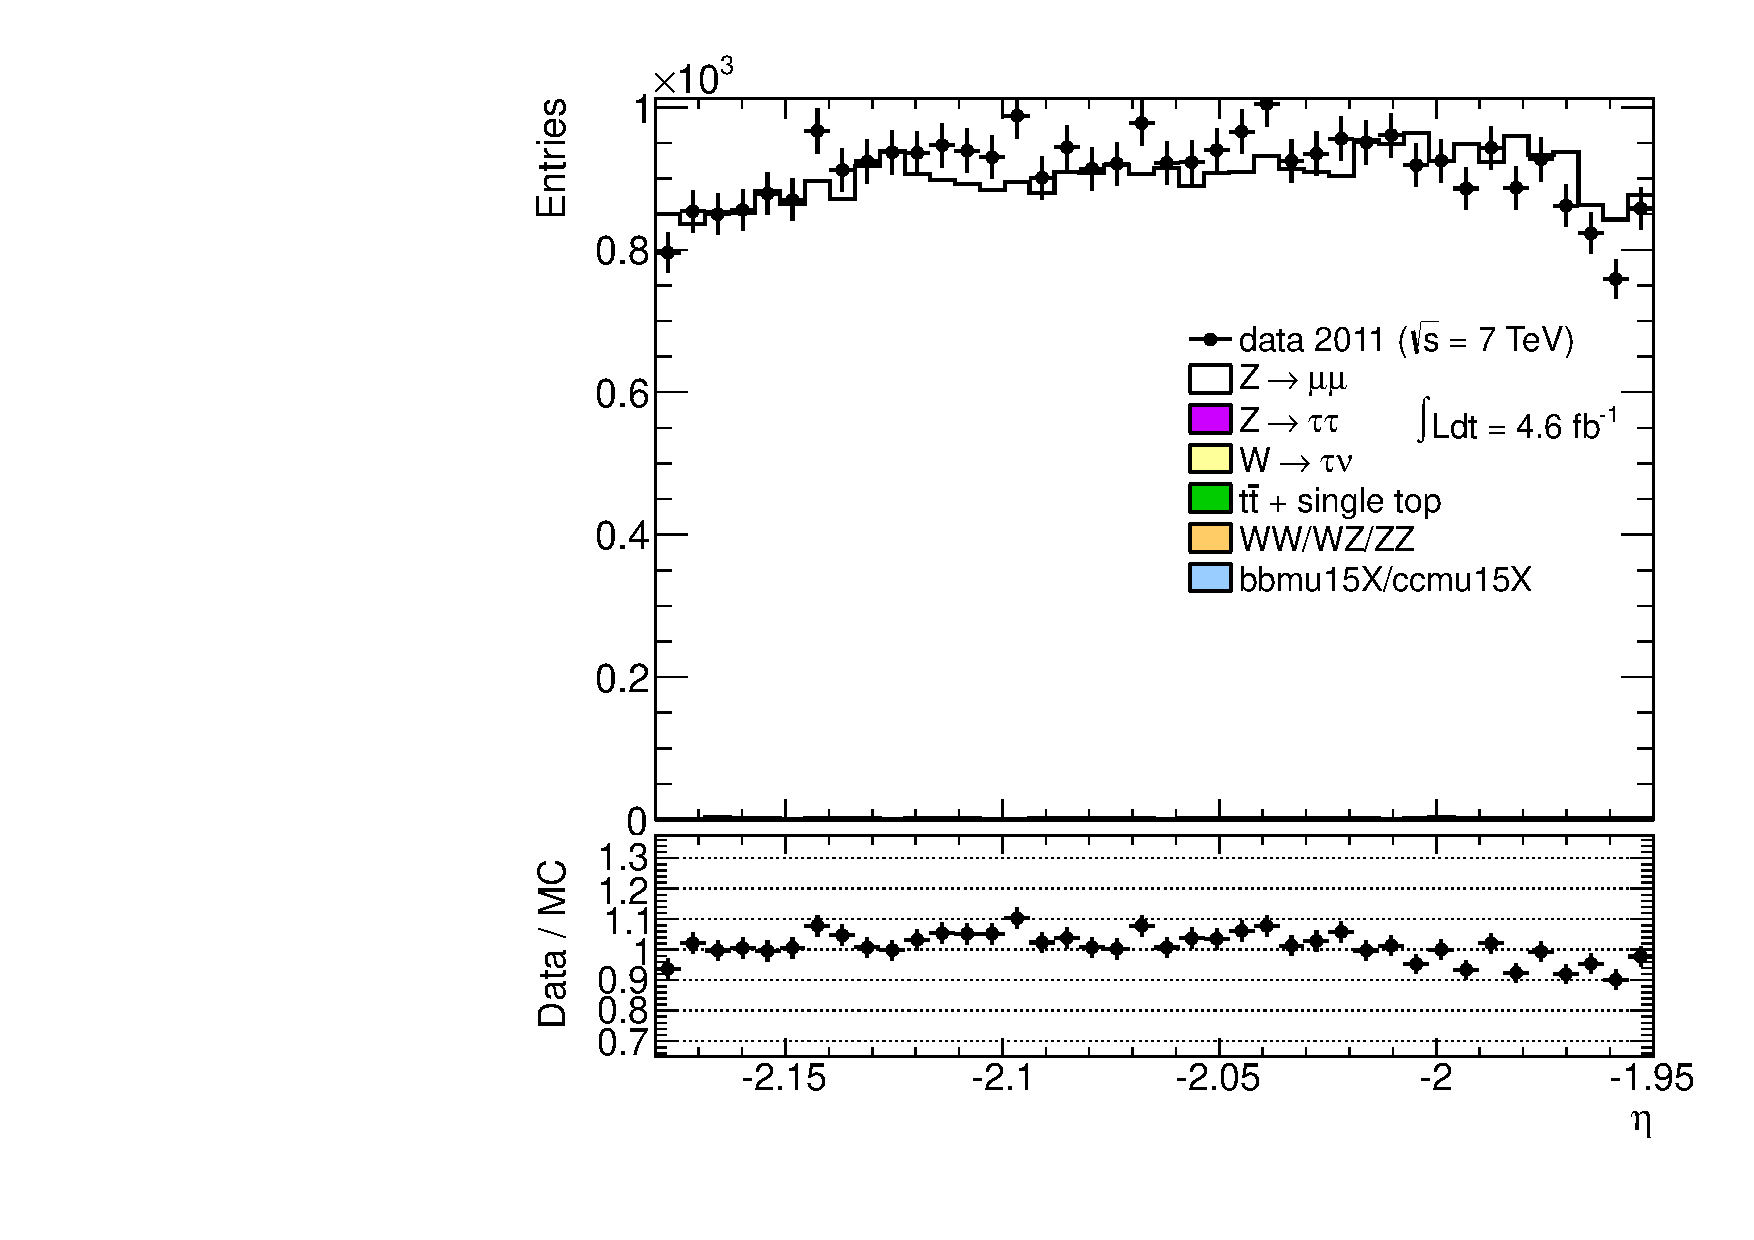
\includegraphics[width=0.66\textwidth]{dates/20130306/figures/both/Z_10_C_stack_lP_eta_ALL.pdf}
\column{.5\textwidth}
A-side $\mu^{+}$ (top: W; bottom: Z)
\centering
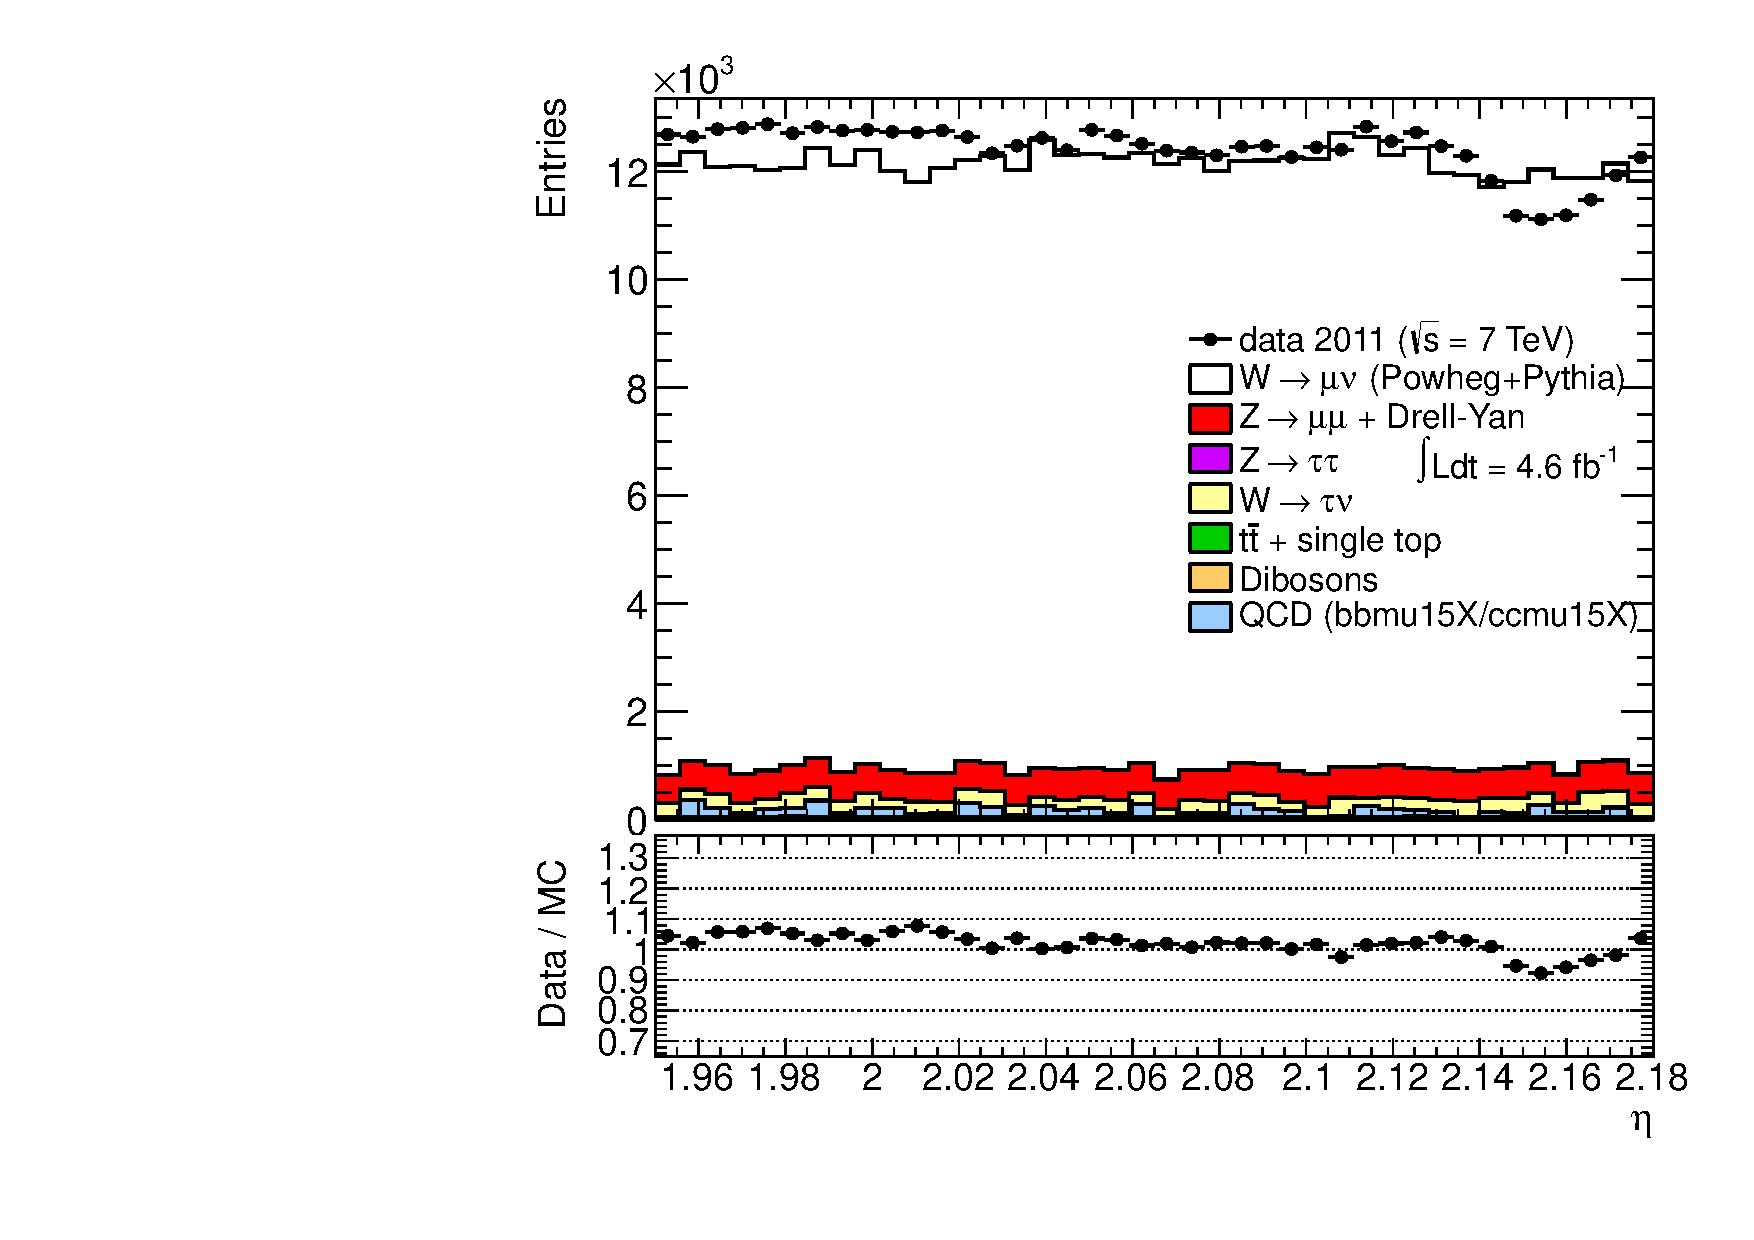
\includegraphics[width=0.66\textwidth]{dates/20130306/figures/both/W_10_A_stack_l_eta_POS} \\
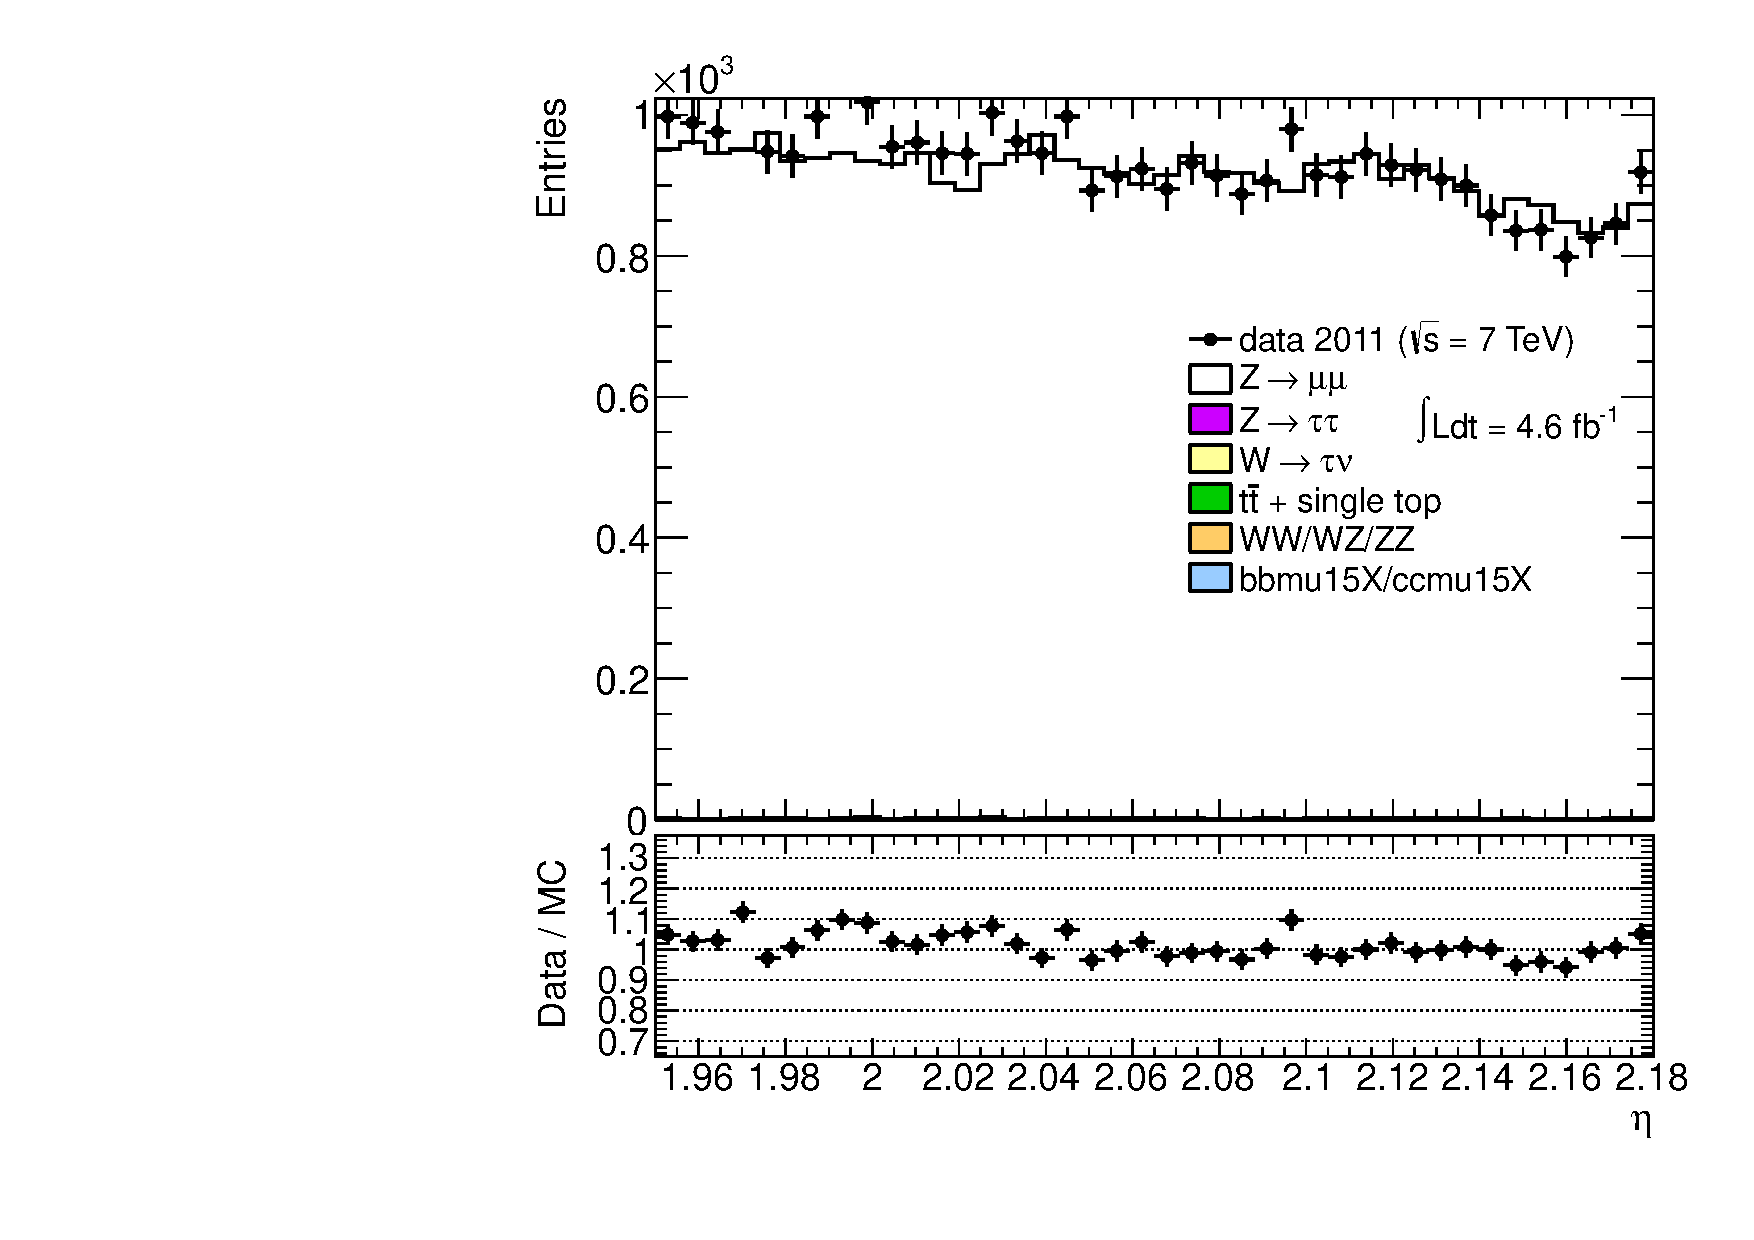
\includegraphics[width=0.66\textwidth]{dates/20130306/figures/both/Z_10_A_stack_lP_eta_ALL.pdf} 
\cole
}
\slide{ Conclusion on A/C problem  }
{
The underlying problem in MG triggers and trigger mathing was reported to trigger experts. \\
In the meanwhile, we switched to mu18 chains because muid triggers are not affected.
}


\slide{ Uncorrelated QCD uncertainty }
{
Statistical uncertainty from QCD fits was:
\iteb
\item treated as correlated across bins
\item added in quadrature with real systematic effects (e.g, fit range, anti-isolation)
\itee
Uncorrelated component has been factored out and included in BackgroundStatisticalUncertainty. \\
E.g., for most central bin, uncorrelated uncertainties on final cross-section are:
\iteb
\item Stat. Uncertainty = 0.14\% (data statistics)
\item Stat. Uncertainty (MC) = 0.12\% (response matrix statistics)
\item Stat. Background = \red{$0.07\% \rightarrow 0.12\%$} (background statistics)
\itee
}

\slide{ Change in Wpt and QCD uncertainty }
{
Best visualized on a plot. \\
Single-differential uncertainties: next slide \\
Double-differential uncertainties: backup
}

\slide{ Single-differential uncertainties }
{
\colb[T]
\column{.5\textwidth}
\centering
\only<1>{ \small{ $W^{-}$: CombinationInputs v8} }
\only<2>{ \small{ $W^{-}$: CombinationInputs vX} }
\includegraphics[width=1.0\textwidth]<1>{dates/20130418/figures/v21/Wmn_SYSTEM_1D_PT25_NEG_Unc_proj}
\includegraphics[width=1.0\textwidth]<2>{dates/20130418/figures/v23/Wmn_SYSTEM_1D_PT25_NEG_Unc_proj}
\column{.5\textwidth}

\centering
\only<1>{ \small{ $W^{+}$: CombinationInputs v8} }
\only<2>{ \small{ $W^{+}$: CombinationInputs vX} }
\includegraphics[width=1.0\textwidth]<1>{dates/20130418/figures/v21/Wmn_SYSTEM_1D_PT25_POS_Unc_proj}
\includegraphics[width=1.0\textwidth]<2>{dates/20130418/figures/v23/Wmn_SYSTEM_1D_PT25_POS_Unc_proj}
\cole
}

\slide{ Overview of Wmunu measurement }
{
Selection, cutflow, control plots, results.
}

\slide{ Selection }
{
  \iteb
  \item \textit{Single muon triggers}: EF\_mu18 or EF\_mu18\_medium
  \item Primary vertex with $\ge$ 3 tracks
  \item Reject events with $BadLooser$ jets or jets in $LarHole$ region
  \item Combined STACO muons passing MCP quality cuts and $|z_0|~<~10~mm$
  \item Muon kinematics: $p_T~>~20~\GeV$ ($25~\GeV$) and $|\eta|~<~2.4$
  \item Tracking isolation: $\sum \pt(\Delta R~<~0.4) / \pt~<~0.1$
  \item \textit{Exactly one isolated muon}
  \item $\met > 25\,\GeV$, $m_{T} > 40\,\GeV$ using \texttt{MET\_RefFinal}
  \itee
}

\slide{ Cutflow }
{
\begin{table}
\footnotesize
\begin{center}
\input{/home/antonk/SupportingDocument/Wmunu/figures/cutflow/data_pt25.tex}
\caption{\it Cutflow for \Wmn\ candidate events in data ($p_T~>~25~\GeV$). Data events that don't have at least one 8 \GeV muon (of any kind) were dropped at the ntuple skimming stage.}
\end{center}
\end{table}
}

\slide{ Backgrounds }
{
\iteb
\item Small backgrounds from other \Zll\ and \Wln\ channels, Dibosons,
  $t\bar{t}$ and single $t$ are estimated with the usual MCs
\iteb
  \item $1-12\%$ depending on $\eta$ and $p_T$ bin (mostly \Wtau\ and \Zll)
\itee
\item Data-driven multi-jet QCD obtained from template fits
\iteb
\item Nominal: \MET fit using ``anti-isolation window'' control region
\item About a dozen systematics: signal, control templates; fit method and variable
\itee
\itee

\centering
\includegraphics[width=0.5\textwidth]{/home/antonk/SupportingDocument/Wmunu/figures/qcdfits/Q0_x_2_2_y_2_7}

}

\slide{ Background fractions - single differential }
{
\begin{figure}[phtb]
  \begin{center}
        \subfigure[QCD uncertainty / $N_{Expected}$: $W^+$]{%
          \includegraphics[width=0.45\textwidth]{/home/antonk/SupportingDocument/Wmunu/figures/qcdunc/Q0_qcd_ptALL25_etaLOOP_ewk_frac}
        } 
       \subfigure[QCD uncertainty / $N_{Expected}$: $W^-$]{%
         \includegraphics[width=0.45\textwidth]{/home/antonk/SupportingDocument/Wmunu/figures/qcdunc/Q1_qcd_ptALL25_etaLOOP_ewk_frac}
        } \\
    \caption{Fractions of QCD and electroweak backgrounds in per cent for the single-differential measurement with muon $p_{T} > 25 GeV$
      in the $W^+$ (left) and $W^-$ (right) channels. The error bars correspond to the total  (statistical  $\oplus$ systematic) uncertainties.}
 \end{center}
\end{figure}
}

\slide{ Background fractions - double differential }
{
\begin{figure}[phtb]
  \begin{center}
   \subfigure[QCD uncertainty / $N_{Expected}$: $W^+$]{%
      \includegraphics[width=0.45\textwidth]{/home/antonk/SupportingDocument/Wmunu/figures/qcdunc/Q0_qcd_adrian_ewk_frac}
      }
       \subfigure[QCD uncertainty / $N_{Expected}$: $W^-$]{%
      \includegraphics[width=0.45\textwidth]{/home/antonk/SupportingDocument/Wmunu/figures/qcdunc/Q1_qcd_adrian_ewk_frac}
      }
    \caption{Fraction of QCD and electroweak backgrounds in per cent for the double-differential measurements
      in the $W^+$ (left) and $W^-$ (right) channels. The error bars correspond to the total  (statistical  $\oplus$ systematic) uncertainties.}
  \end{center}
\end{figure}

}

\slide{Control plots}
{
\only<1>{$\Wminus  \rightarrow \mu^-\nu$}
\only<2>{$\Wplus  \rightarrow \mu^{+} \nu$}
\scriptsize{(Systematic band includes all experimental uncertainties + MC generators + boson $p_{T}$.)}

\vspace{-.3cm}
 \begin{columns}
  \begin{column}{0.32\textwidth}
     \begin{center}
       Muon $\eta$ \\
       \vspace{-.03cm}
       \includegraphics[width=1.00\textwidth]<1>{/home/antonk/SupportingDocument/Wmunu/figures/control_plots/inclusive25/P_stack_d3_eta_lpt_met_y_2__1_z_0__1_NEG}
       \includegraphics[width=1.00\textwidth]<2>{/home/antonk/SupportingDocument/Wmunu/figures/control_plots/inclusive25/P_stack_d3_eta_lpt_met_y_2__1_z_0__1_POS}
     \end{center}
     \vspace{-.7cm}
     \begin{center}
       Muon $p_T$ \\
       \vspace{-.03cm}
       \includegraphics[width=1.00\textwidth]<1>{/home/antonk/SupportingDocument/Wmunu/figures/control_plots/inclusive25/P_stack_lpt_NEG}
       \includegraphics[width=1.00\textwidth]<2>{/home/antonk/SupportingDocument/Wmunu/figures/control_plots/inclusive25/P_stack_lpt_POS}
     \end{center}
  \end{column}

  \begin{column}{0.32\textwidth}
     \begin{center}
       $E_T^{Miss}$ \\
       \vspace{-.03cm}
       \includegraphics[width=1.00\textwidth]<1>{/home/antonk/SupportingDocument/Wmunu/figures/control_plots/inclusive25/P_stack_d3_abseta_lpt_met_x_0__1_y_2__1_NEG}
       \includegraphics[width=1.00\textwidth]<2>{/home/antonk/SupportingDocument/Wmunu/figures/control_plots/inclusive25/P_stack_d3_abseta_lpt_met_x_0__1_y_2__1_POS}
     \end{center}
     \vspace{-.7cm}
     \begin{center}
       $m_T^{W}$ \\
       \vspace{-.03cm}
       \includegraphics[width=1.00\textwidth]<1>{/home/antonk/SupportingDocument/Wmunu/figures/control_plots/inclusive25/P_stack_d3_abseta_lpt_wmt_x_0__1_y_2__1_NEG}
       \includegraphics[width=1.00\textwidth]<2>{/home/antonk/SupportingDocument/Wmunu/figures/control_plots/inclusive25/P_stack_d3_abseta_lpt_wmt_x_0__1_y_2__1_POS}
     \end{center}
  \end{column}

  \begin{column}{0.32\textwidth}
     \begin{center}
       $p^{W}_{T}$ \\
       \vspace{-.03cm}
       \includegraphics[width=1.0\textwidth]<1>{/home/antonk/SupportingDocument/Wmunu/figures/control_plots/inclusive25/P_stack_d3_abseta_lpt_wpt_x_0__1_y_2__1_NEG}
       \includegraphics[width=1.0\textwidth]<2>{/home/antonk/SupportingDocument/Wmunu/figures/control_plots/inclusive25/P_stack_d3_abseta_lpt_wpt_x_0__1_y_2__1_POS}
     \end{center}
     \vspace{-.7cm}
     \begin{center}
       $Muon~\phi$ \\
       \vspace{-.03cm}
       \includegraphics[width=1.0\textwidth]<1>{/home/antonk/SupportingDocument/Wmunu/figures/control_plots/inclusive25/P_stack_d3_abseta_lpt_phi_x_0__1_y_2__1_NEG}
       \includegraphics[width=1.0\textwidth]<2>{/home/antonk/SupportingDocument/Wmunu/figures/control_plots/inclusive25/P_stack_d3_abseta_lpt_phi_x_0__1_y_2__1_POS}
     \end{center}
  \end{column}

\end{columns}
}

\slide{ Smoothing of theory systematics - background  }
{
\begin{figure}[phtb]
  \begin{center}
        \subfigure[\tiny{$W+$: PS}]{%
          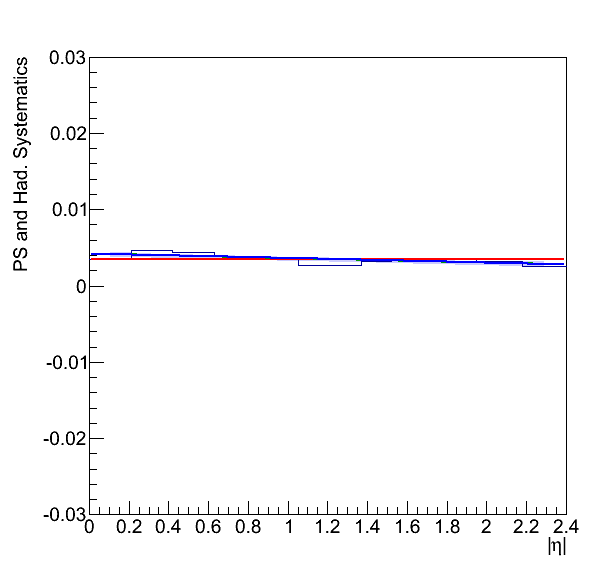
\includegraphics[width=0.27\textwidth]{/home/antonk/SupportingDocument/Wmunu/figures/smoothing/1D_pt25_POS_PSsyst_onlybg}
        } 
       \subfigure[\tiny{$W^-$: PS}]{%
         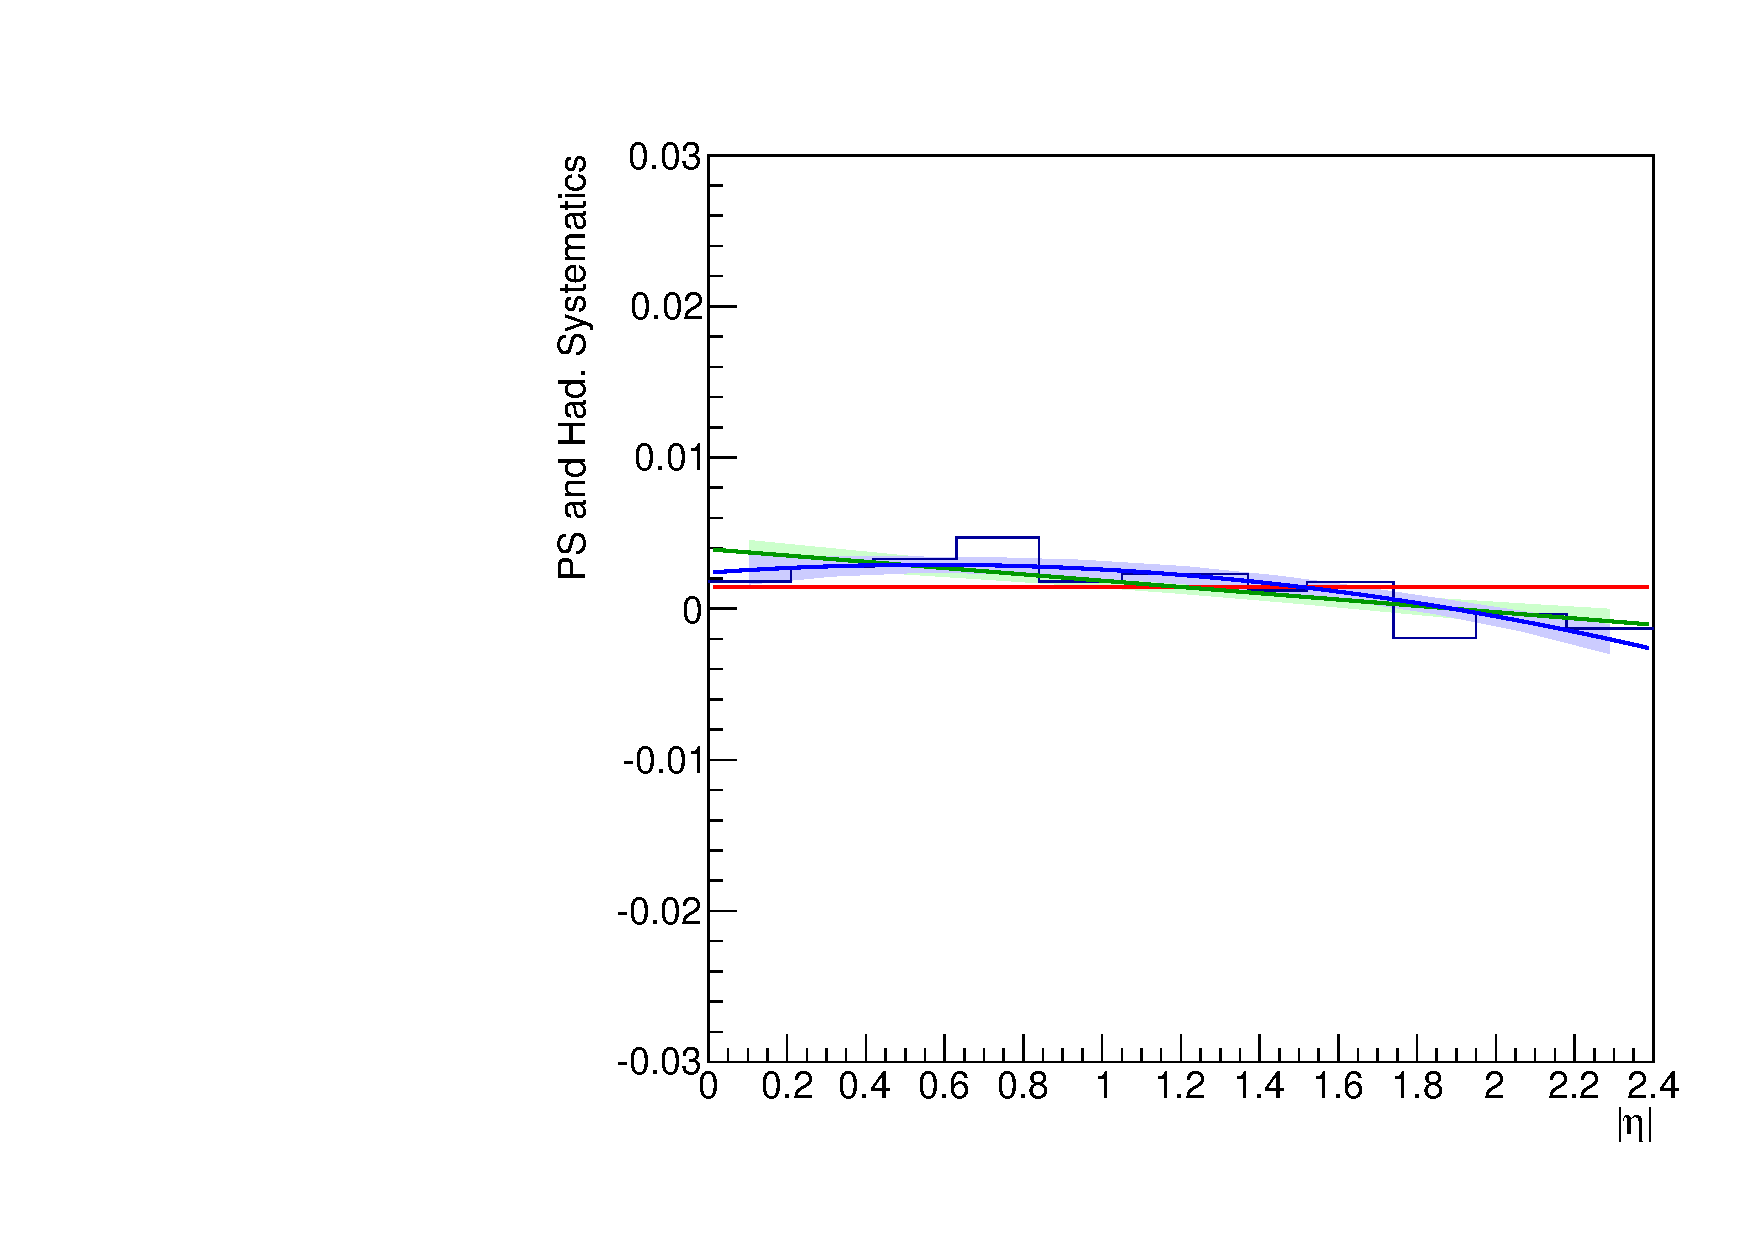
\includegraphics[width=0.27\textwidth]{/home/antonk/SupportingDocument/Wmunu/figures/smoothing/1D_pt25_NEG_PSsyst_onlybg}
        } \\
        \subfigure[\tiny{$W+$: ME}]{%
          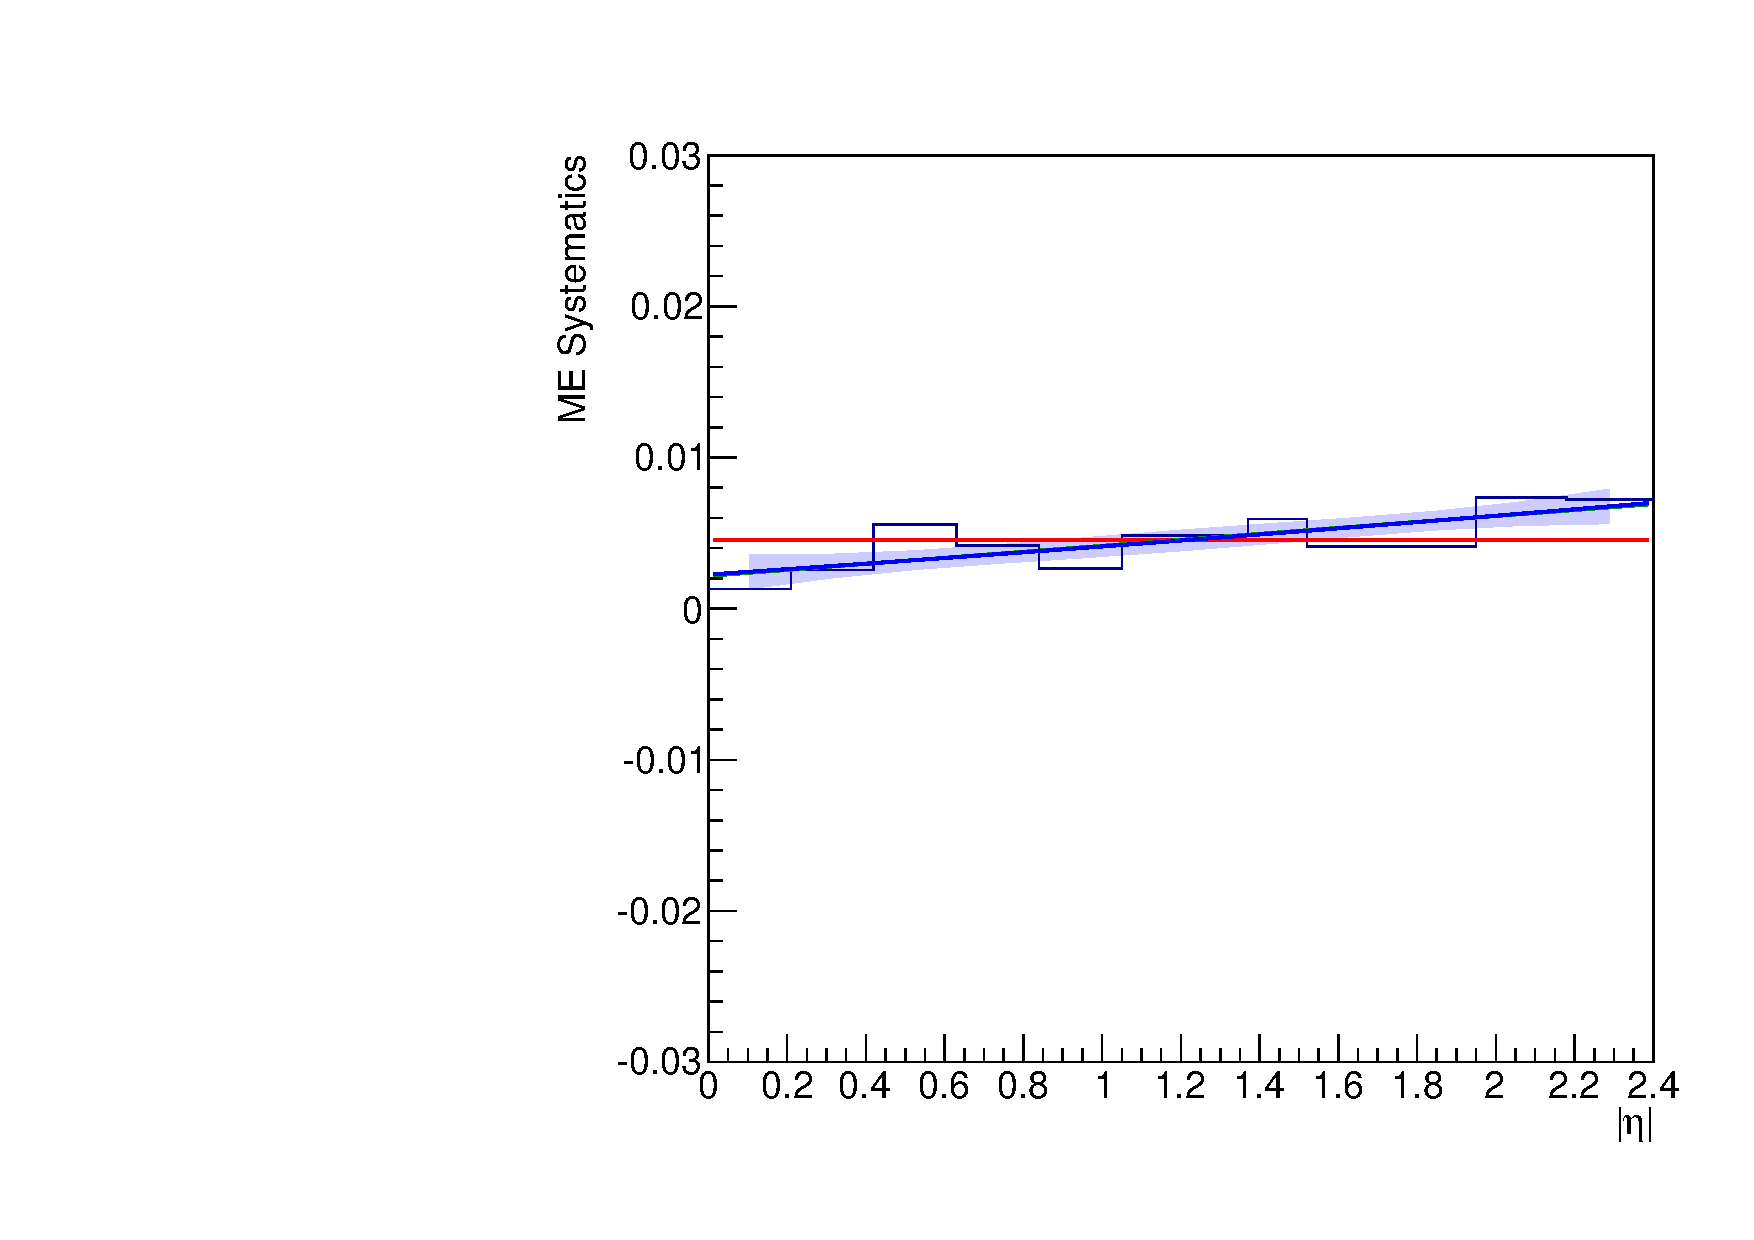
\includegraphics[width=0.27\textwidth]{/home/antonk/SupportingDocument/Wmunu/figures/smoothing/1D_pt25_POS_MEsyst_onlybg}
        } 
       \subfigure[\tiny{$W^-$: ME}]{%
         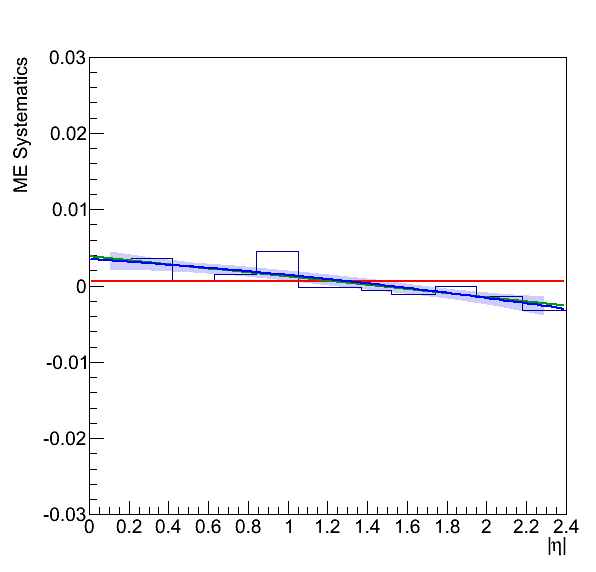
\includegraphics[width=0.27\textwidth]{/home/antonk/SupportingDocument/Wmunu/figures/smoothing/1D_pt25_NEG_MEsyst_onlybg}
        } \\
 \end{center}
\end{figure}
}

\slide{ Smoothing of theory systematics - unfolding  }
{

\begin{figure}[phtb]
  \begin{center}
        \subfigure[\tiny{$W+$: PS}]{%
          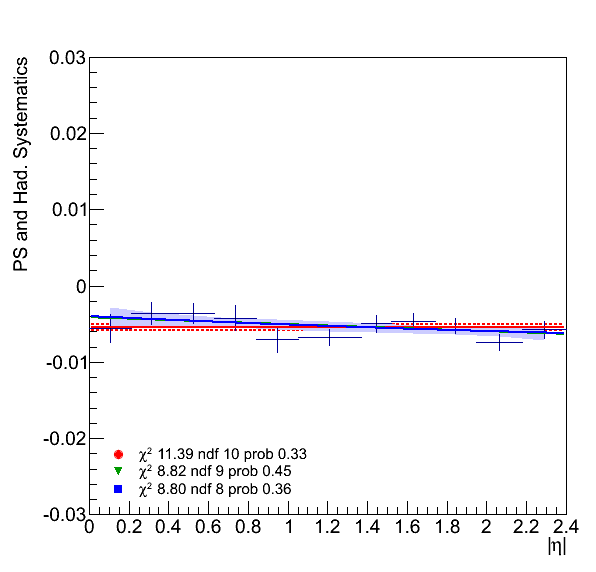
\includegraphics[width=0.27\textwidth]{/home/antonk/SupportingDocument/Wmunu/figures/smoothing/1D_pt25_POS_PSsyst_onlyunf}
        } 
       \subfigure[\tiny{$W^-$: PS}]{%
         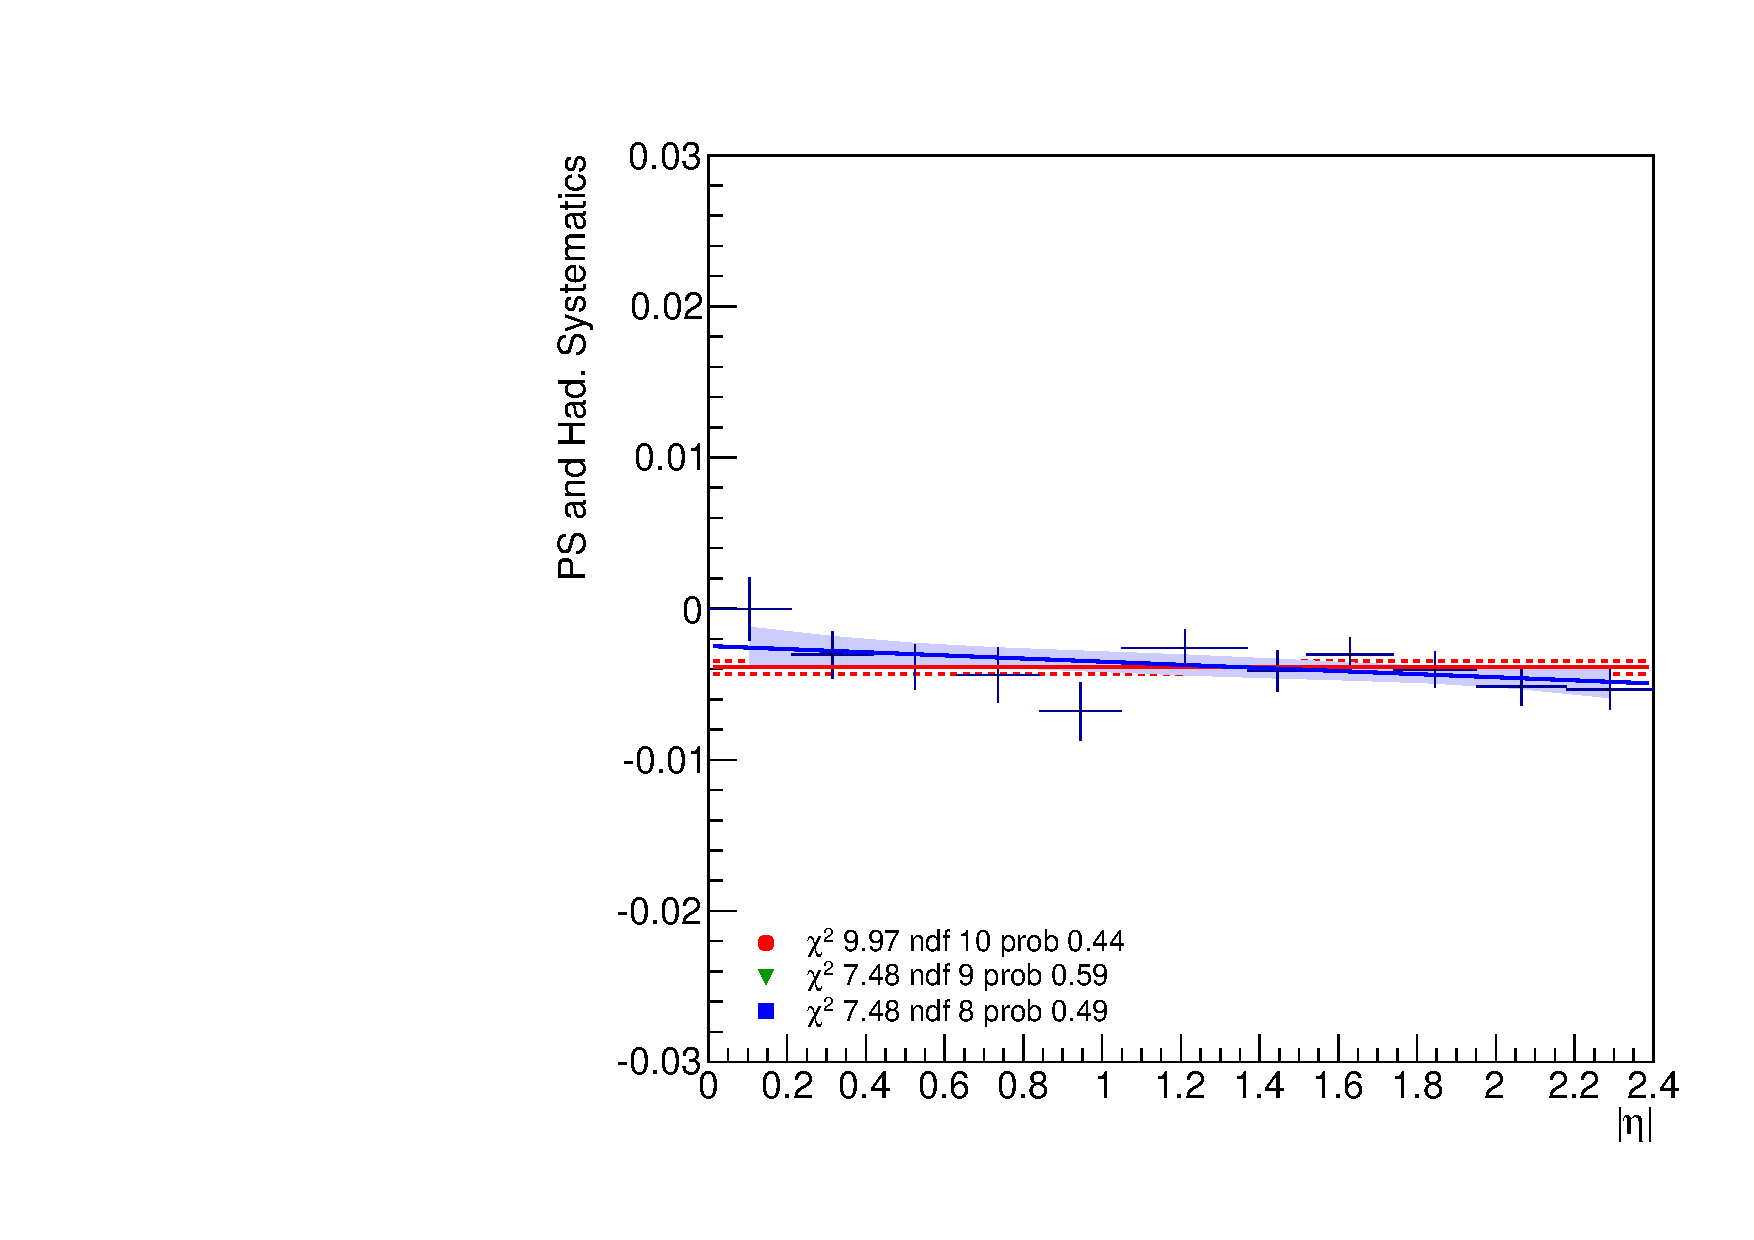
\includegraphics[width=0.27\textwidth]{/home/antonk/SupportingDocument/Wmunu/figures/smoothing/1D_pt25_NEG_PSsyst_onlyunf}
        } \\
        \subfigure[\tiny{$W+$: ME}]{%
          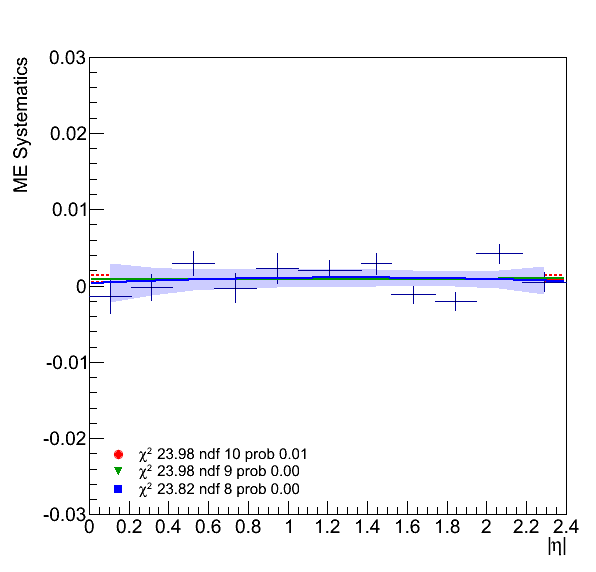
\includegraphics[width=0.27\textwidth]{/home/antonk/SupportingDocument/Wmunu/figures/smoothing/1D_pt25_POS_MEsyst_onlyunf}
        } 
       \subfigure[\tiny{$W^-$: ME}]{%
         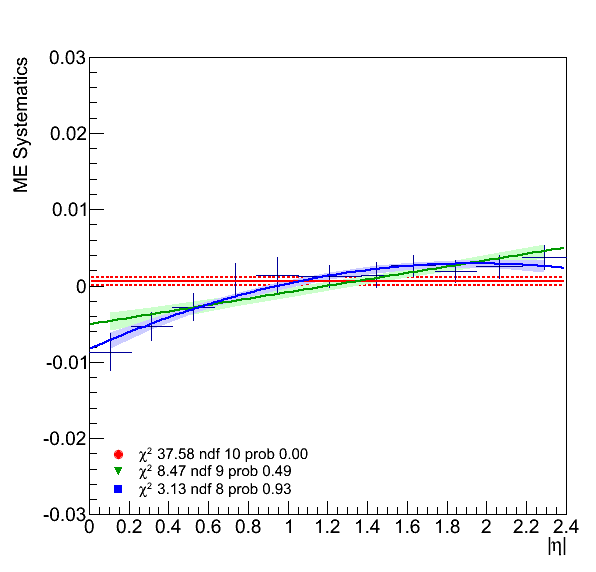
\includegraphics[width=0.27\textwidth]{/home/antonk/SupportingDocument/Wmunu/figures/smoothing/1D_pt25_NEG_MEsyst_onlyunf}
        } \\
 \end{center}
\end{figure}

}

\slide{Results - single differential}
{
\begin{figure}[phtb]
  \begin{center}
        \subfigure[\Wplus]{%
	  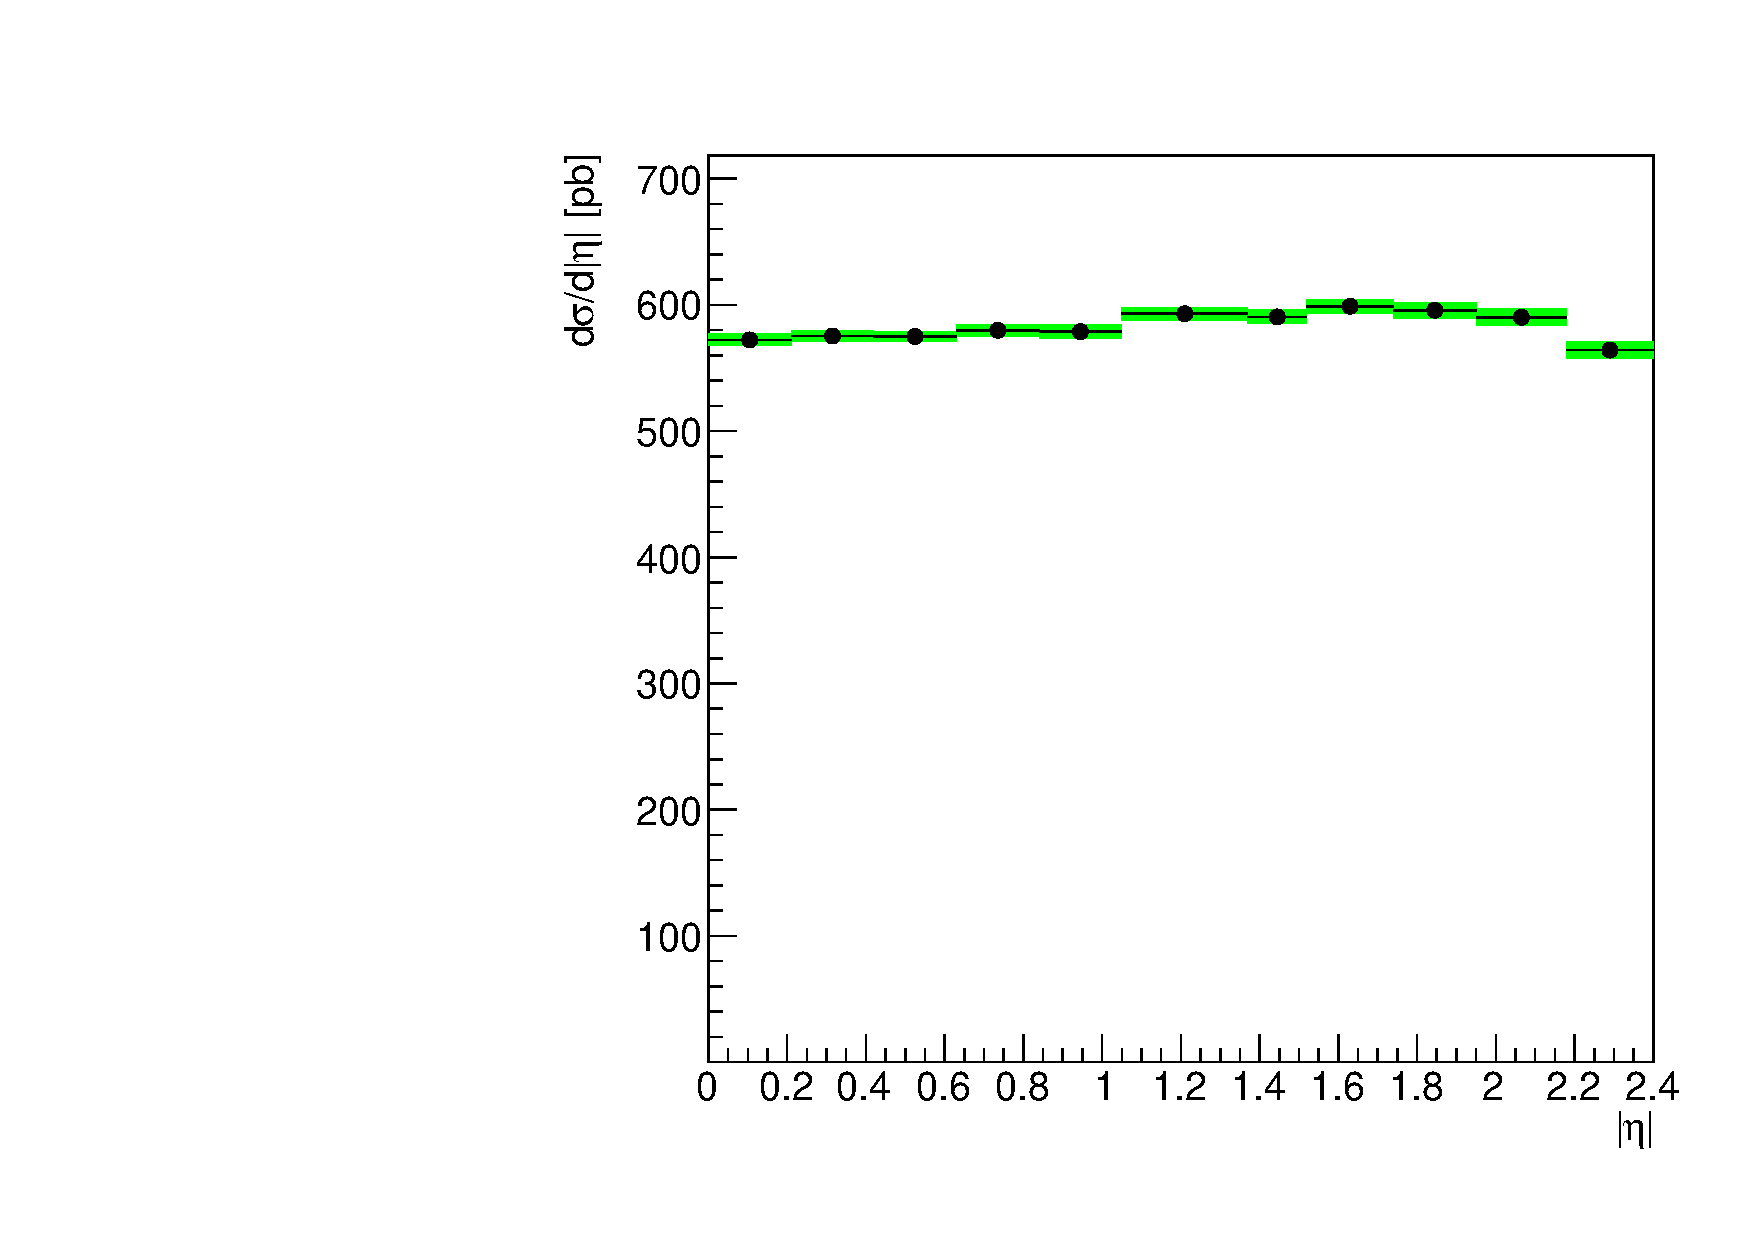
\includegraphics[width=0.4\textwidth]{/home/antonk/SupportingDocument/Wmunu/figures/res/Wmn_UNFABS_1D_PT25_POS_UnfAbs_proj}
        } 
        \subfigure[\Wminus]{%
	  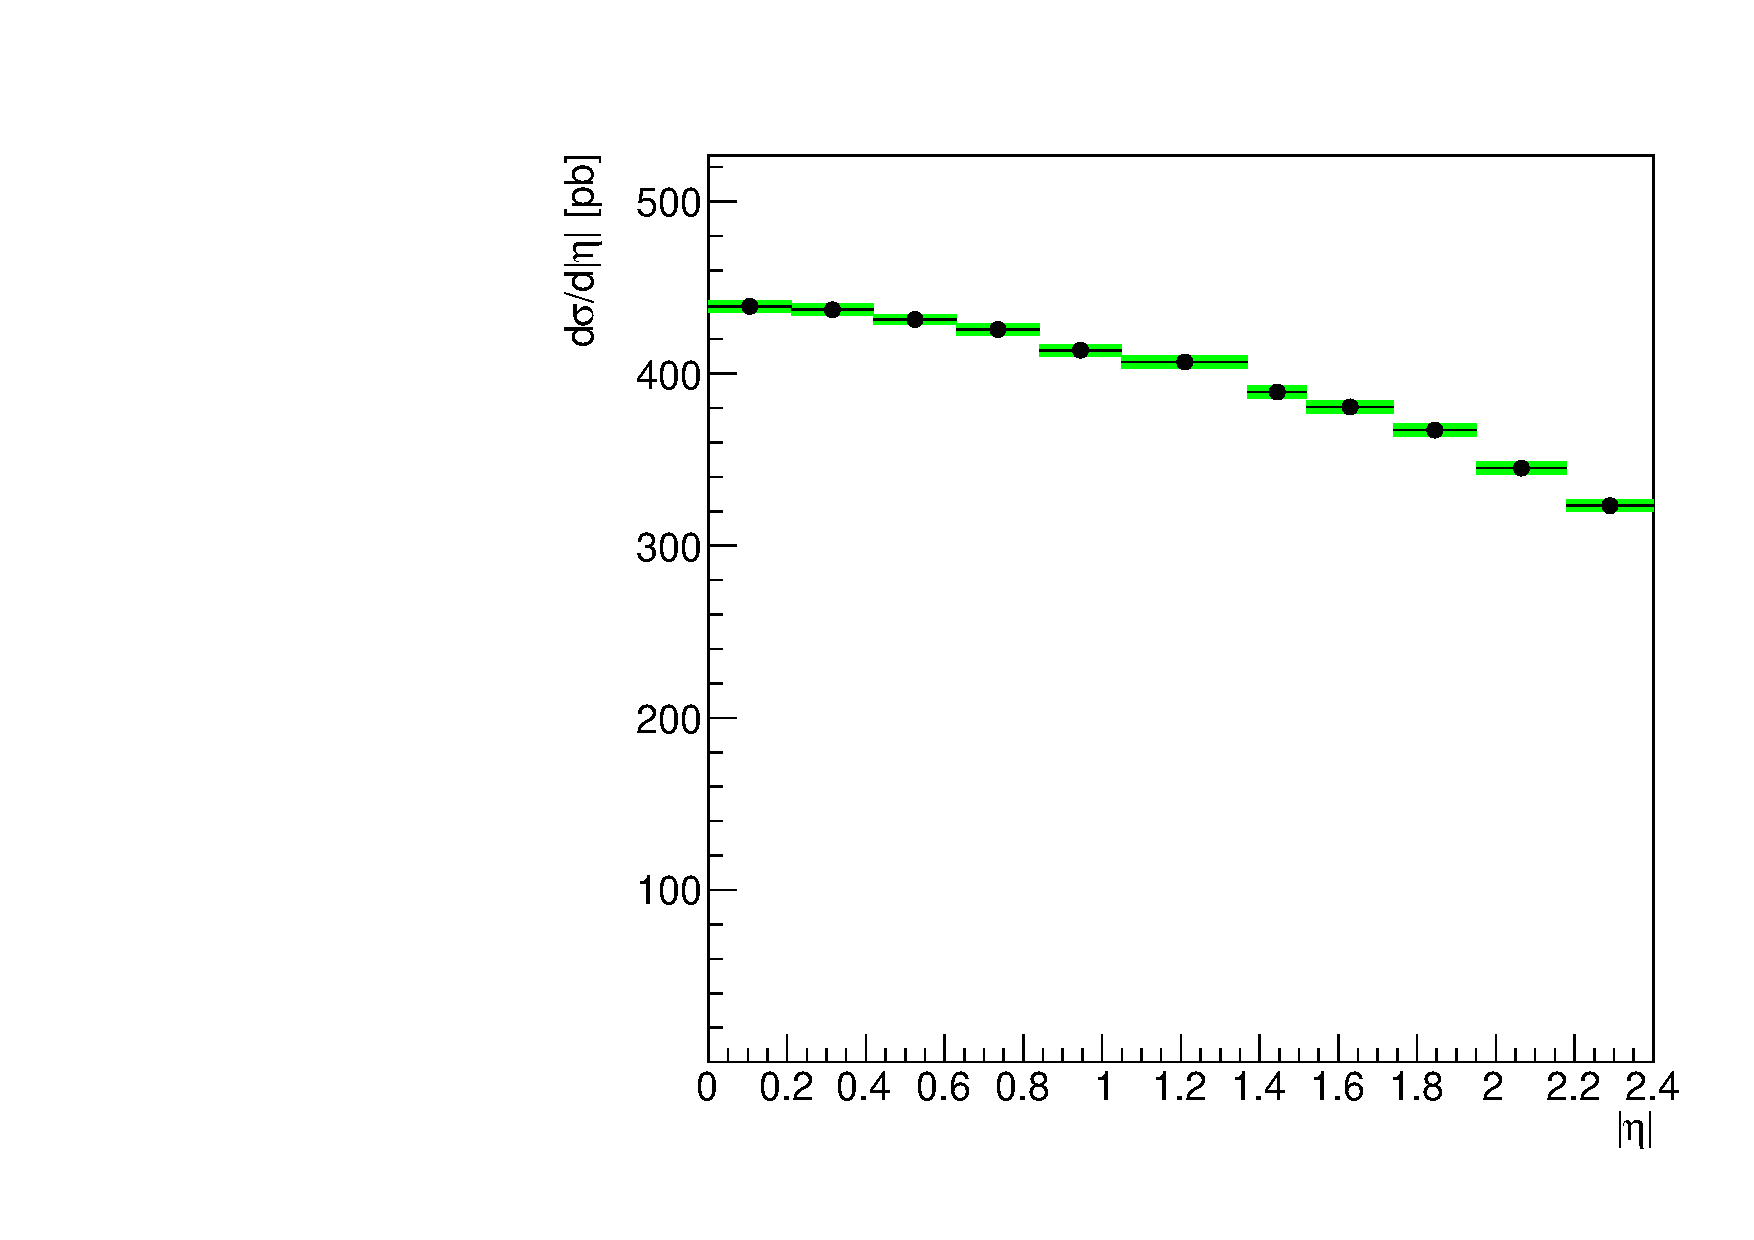
\includegraphics[width=0.4\textwidth]{/home/antonk/SupportingDocument/Wmunu/figures/res/Wmn_UNFABS_1D_PT25_NEG_UnfAbs_proj}
        }
 \caption{\it Absolute single-differential fiducial cross sections in the \Wmunup\ (left) and \Wmunum\ (right) channels ($p_{T}~>~25~\GeV$)}
 \end{center}
\end{figure}
}

\slide{Results - double differential $W^+$}
{
\begin{figure}[phtb]
  \begin{center}
        \subfigure[\ptOne]{%
	  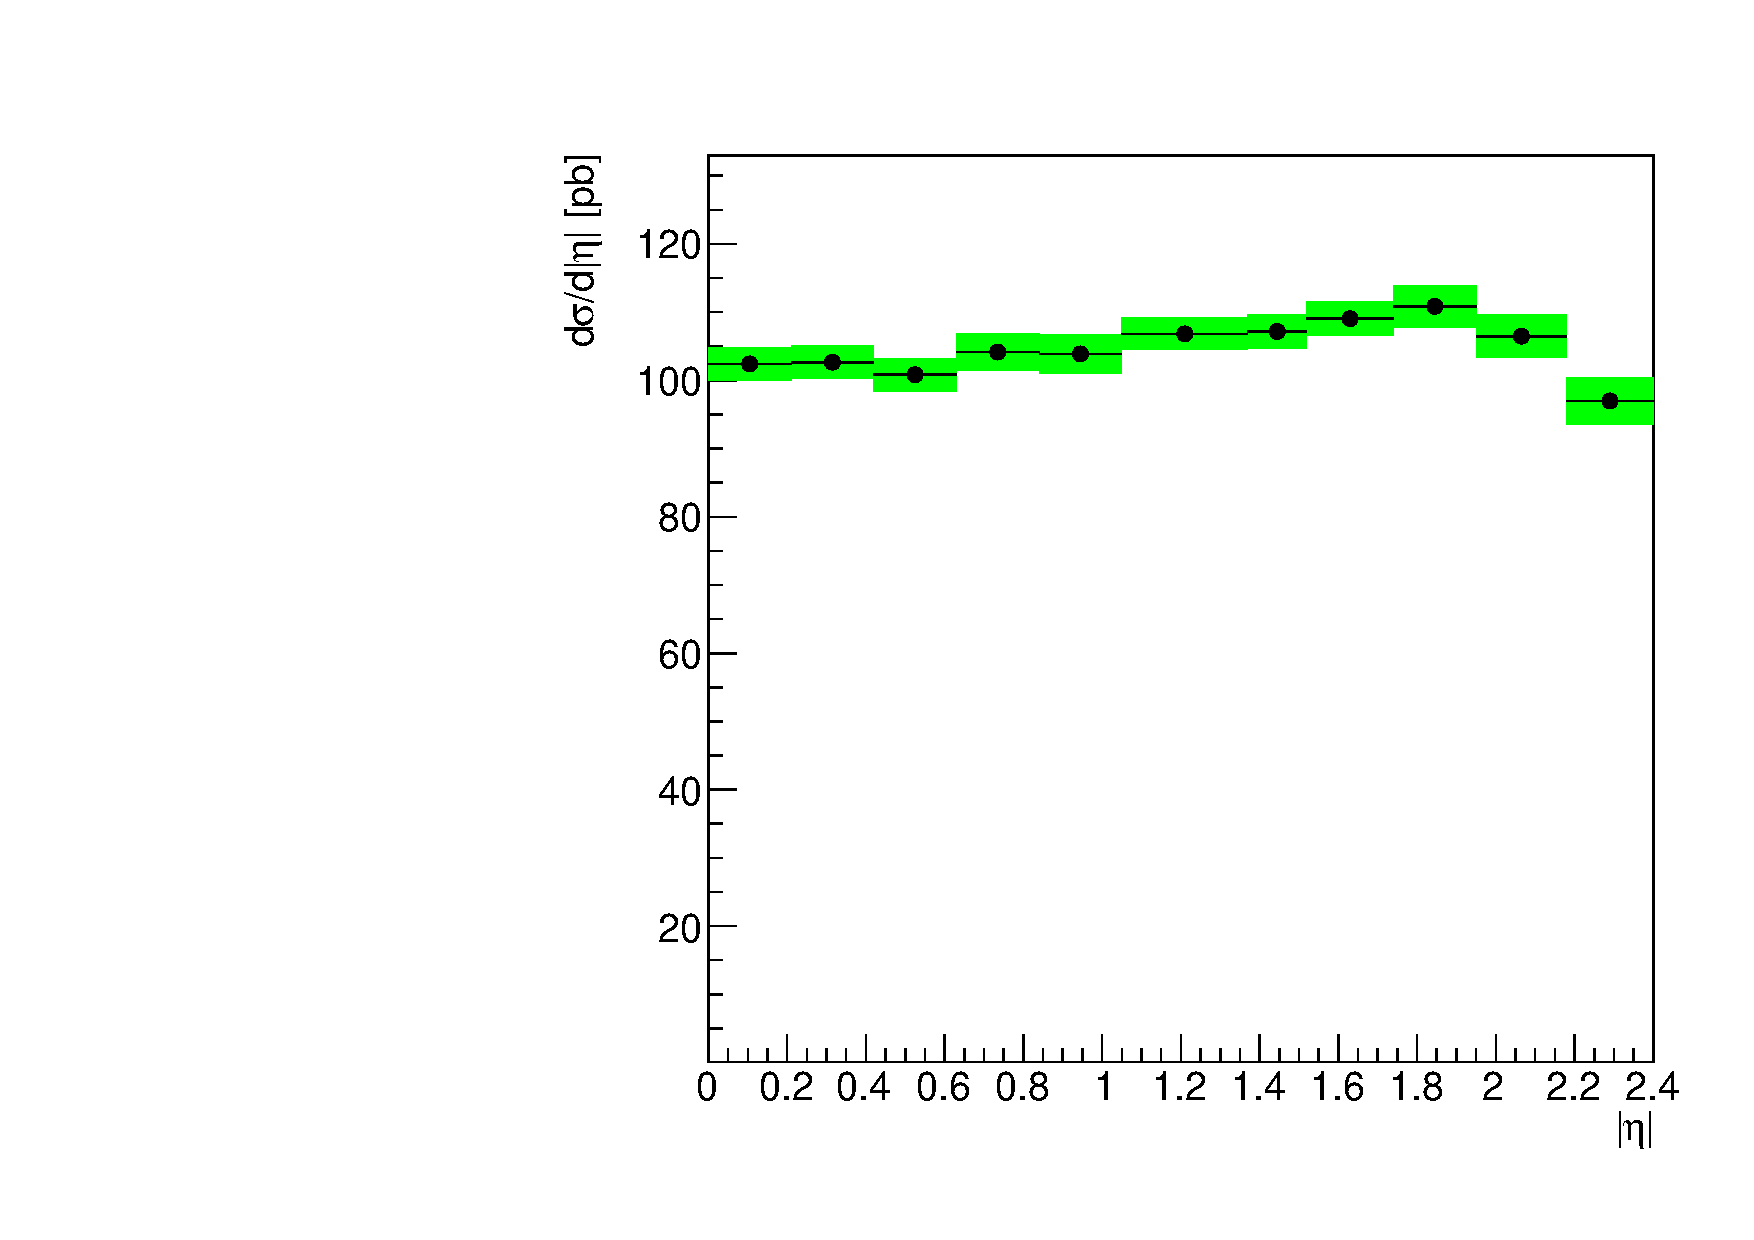
\includegraphics[width=0.27\textwidth]{/home/antonk/SupportingDocument/Wmunu/figures/res/Wmn_UNFABS_2D_PT20_POS_UnfAbs_2d_Slice_2}
        }
       \subfigure[\ptTwo]{%
	  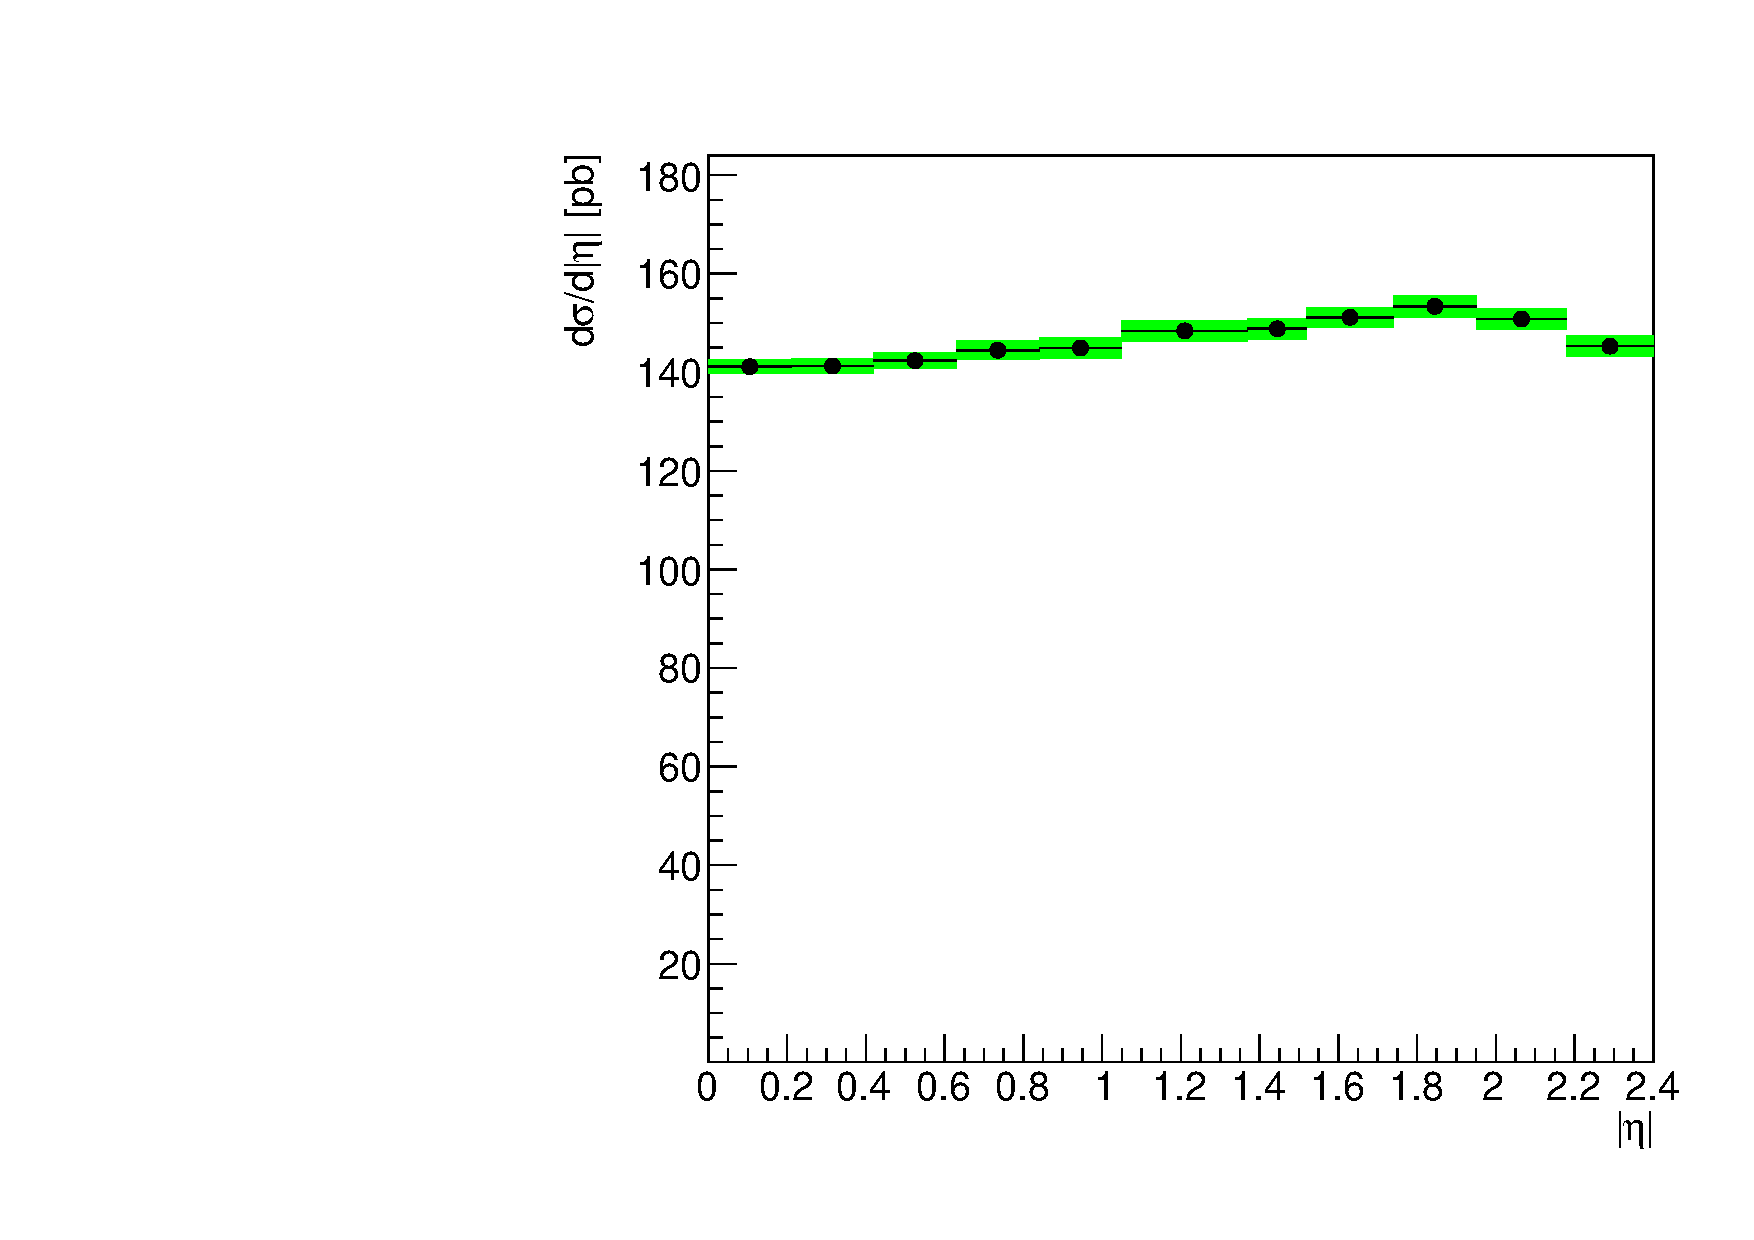
\includegraphics[width=0.27\textwidth]{/home/antonk/SupportingDocument/Wmunu/figures/res/Wmn_UNFABS_2D_PT20_POS_UnfAbs_2d_Slice_3}
        }
       \subfigure[\ptThree]{%
	  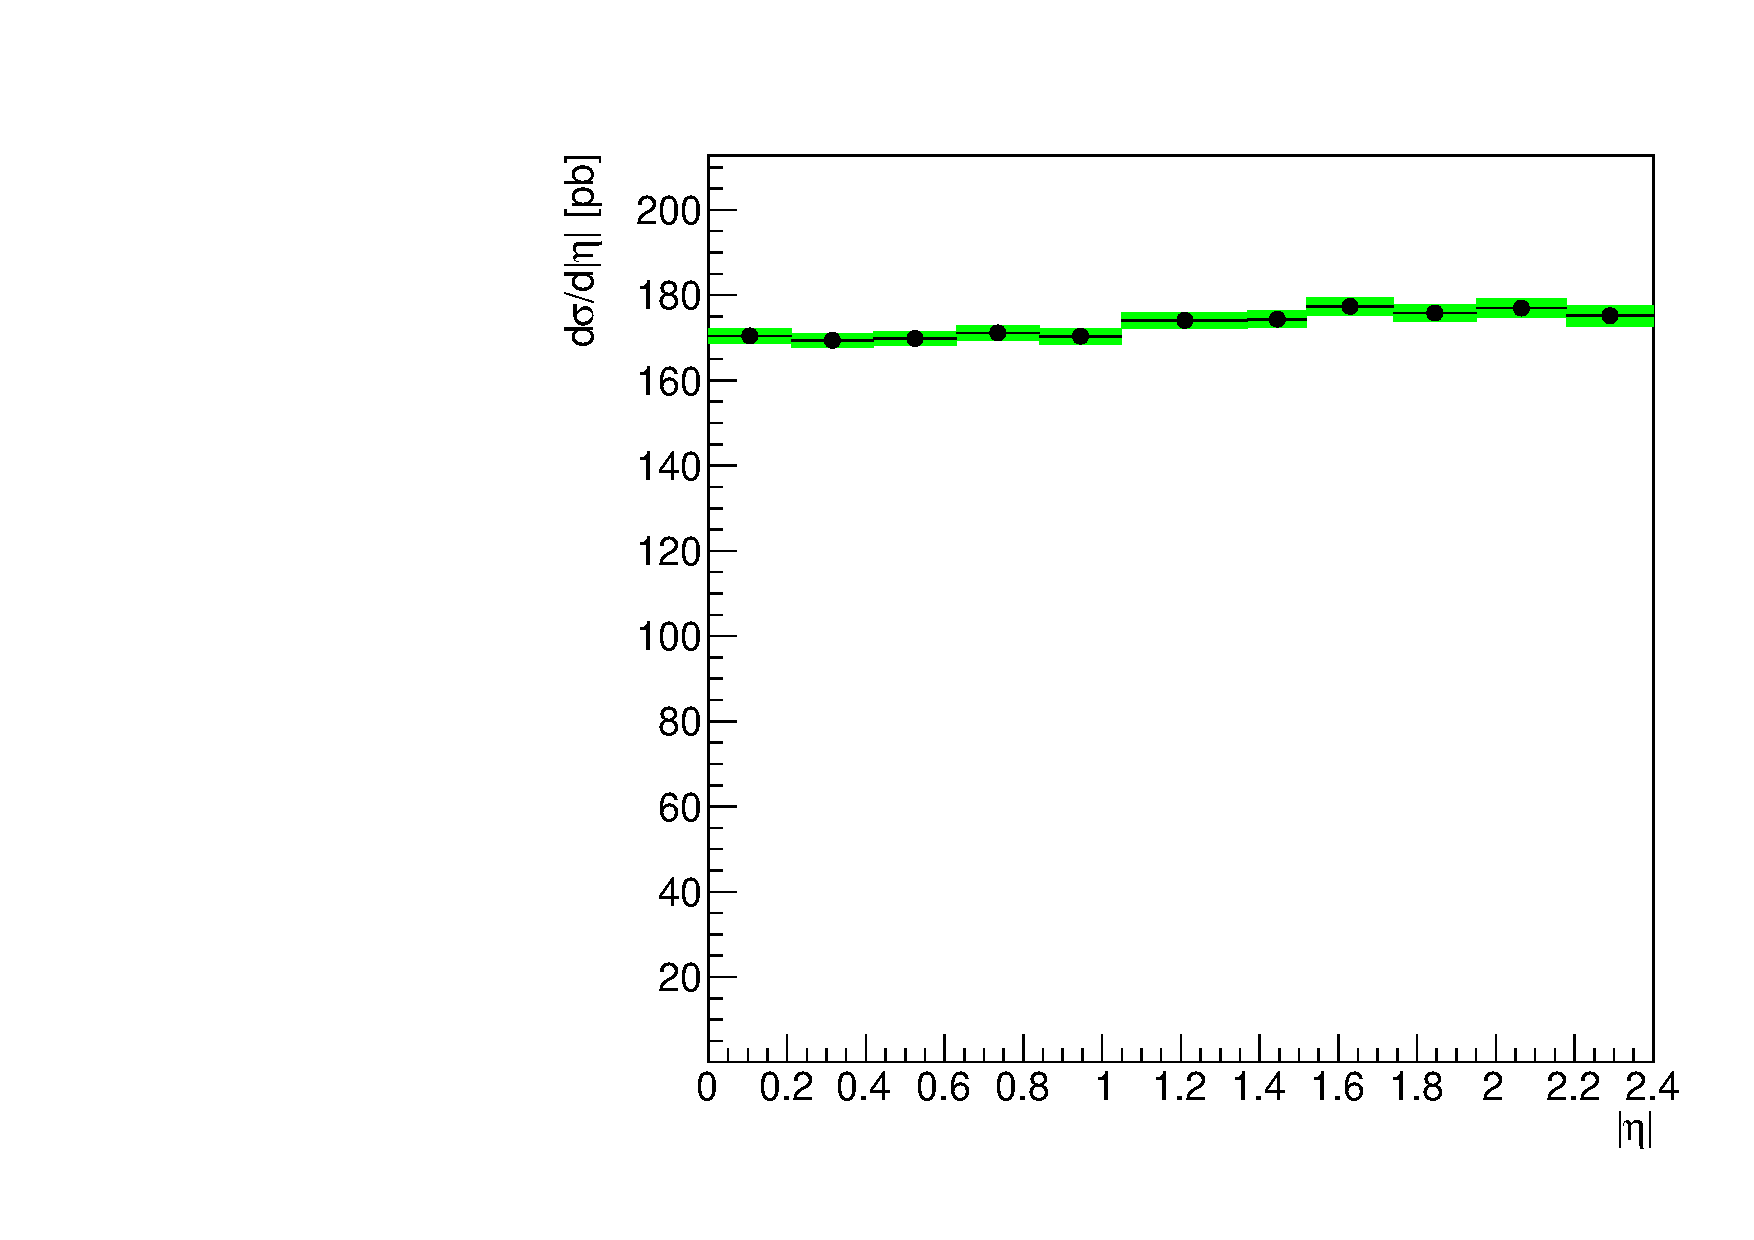
\includegraphics[width=0.27\textwidth]{/home/antonk/SupportingDocument/Wmunu/figures/res/Wmn_UNFABS_2D_PT20_POS_UnfAbs_2d_Slice_4}
        } \\
       \subfigure[\ptFour]{%
	  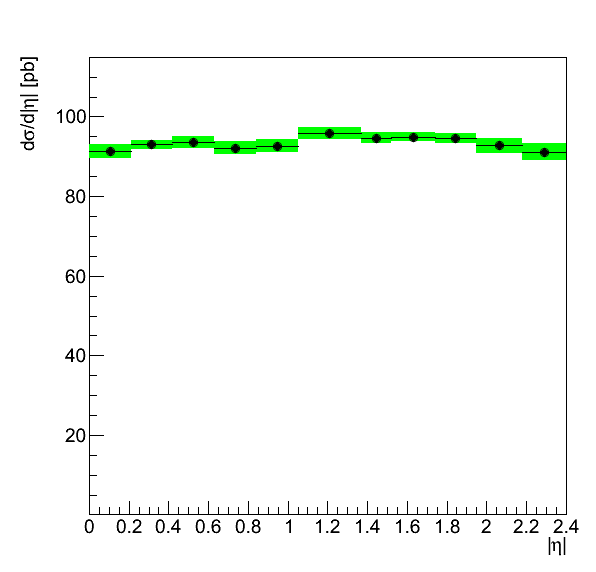
\includegraphics[width=0.27\textwidth]{/home/antonk/SupportingDocument/Wmunu/figures/res/Wmn_UNFABS_2D_PT20_POS_UnfAbs_2d_Slice_5}
        }
       \subfigure[\ptFive]{%
	  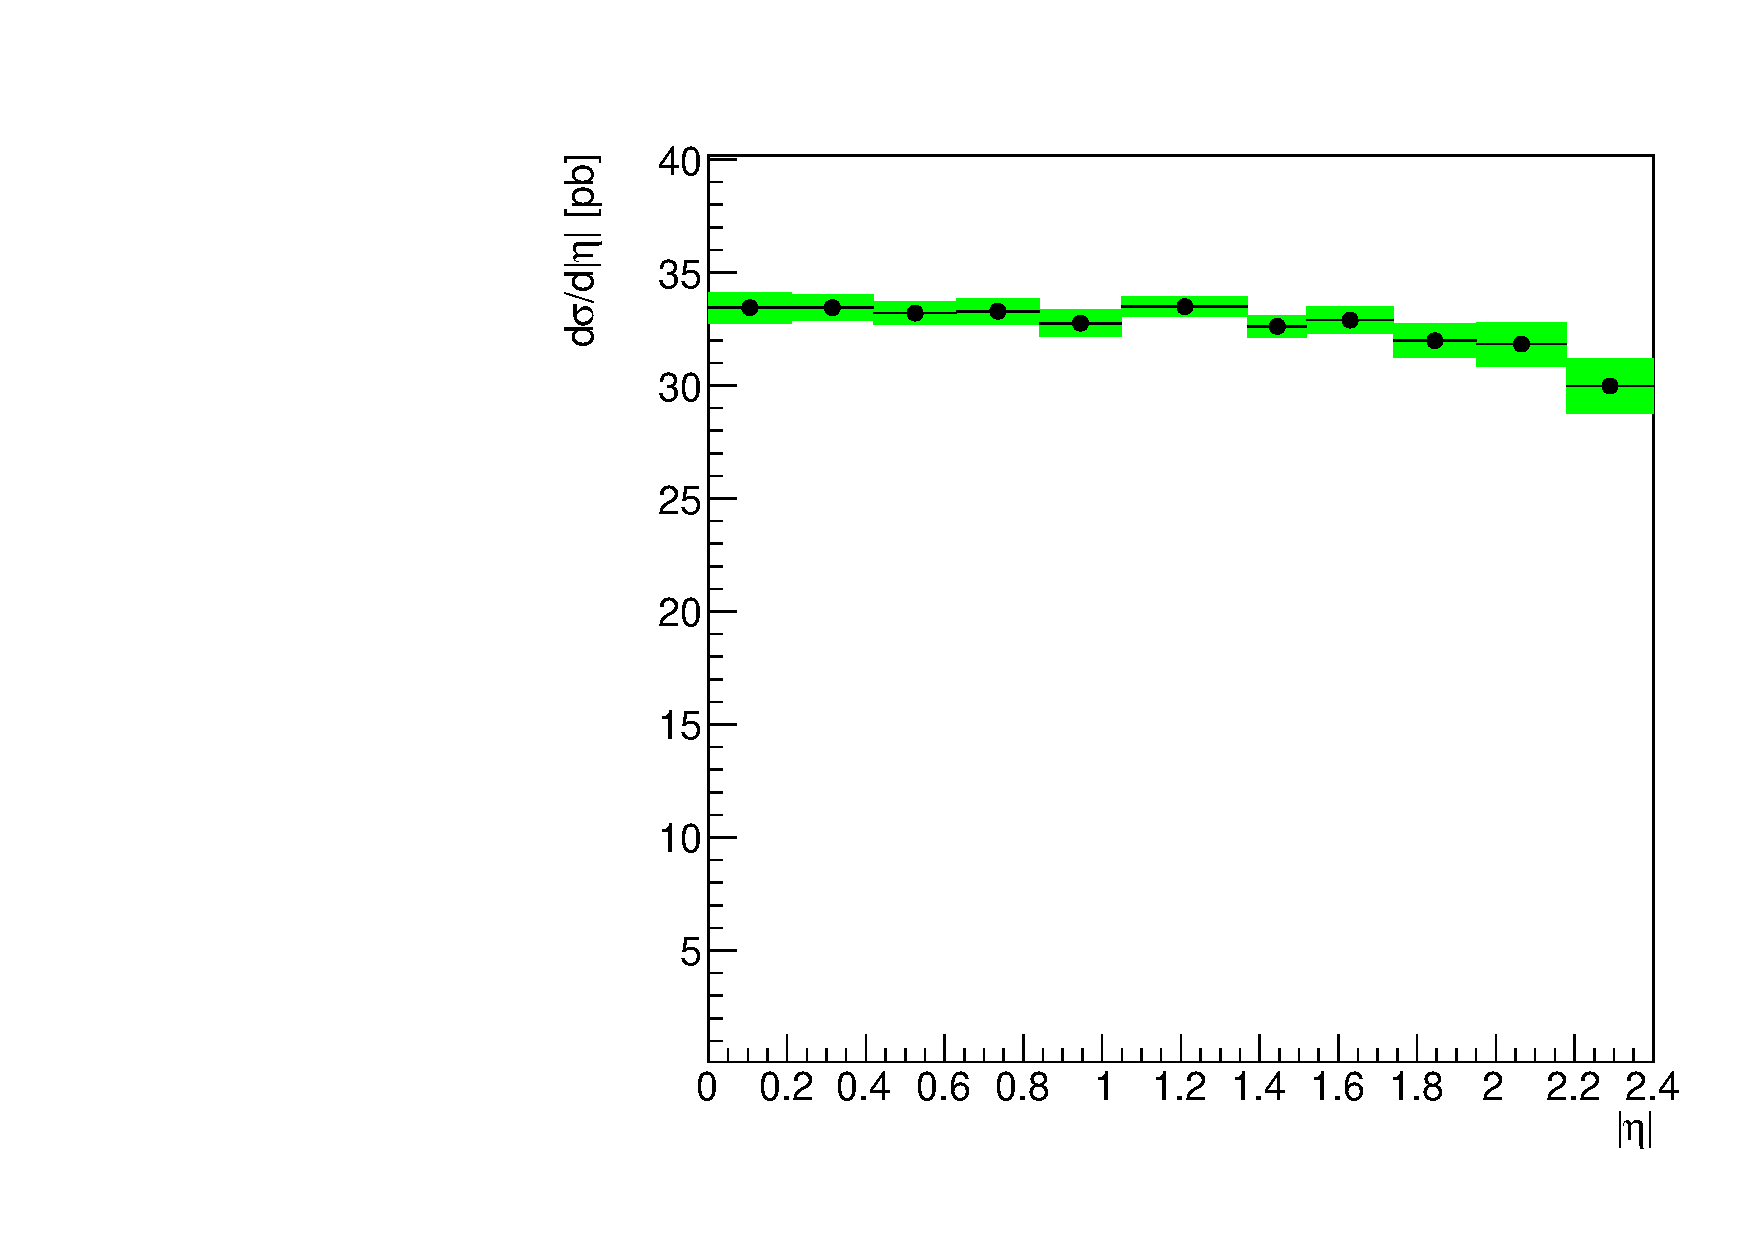
\includegraphics[width=0.27\textwidth]{/home/antonk/SupportingDocument/Wmunu/figures/res/Wmn_UNFABS_2D_PT20_POS_UnfAbs_2d_Slice_6}
        }
       \subfigure[\ptSix]{%
	  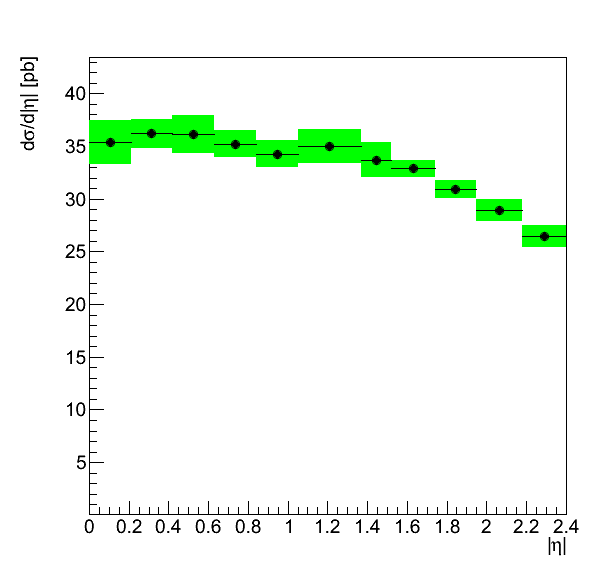
\includegraphics[width=0.27\textwidth]{/home/antonk/SupportingDocument/Wmunu/figures/res/Wmn_UNFABS_2D_PT20_POS_UnfAbs_2d_Slice_7}
       } 
 \end{center}
\end{figure}
}

\slide{Results - double differential $W^-$}
{
\begin{figure}[phtb]
  \begin{center}
        \subfigure[\ptOne]{%
	  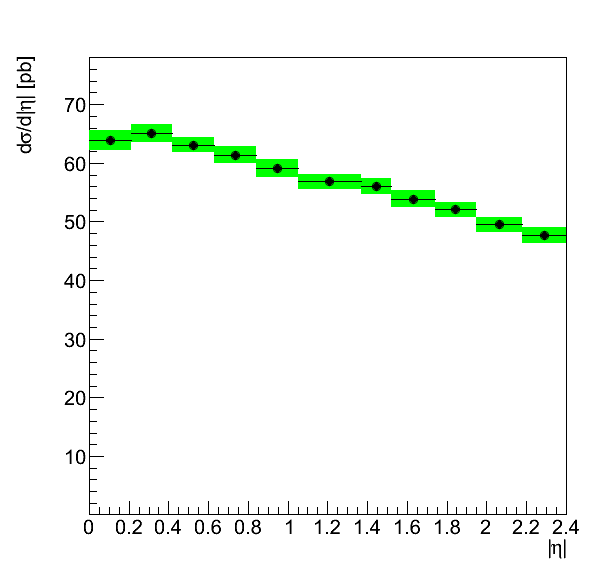
\includegraphics[width=0.27\textwidth]{/home/antonk/SupportingDocument/Wmunu/figures/res/Wmn_UNFABS_2D_PT20_NEG_UnfAbs_2d_Slice_2}
        }
       \subfigure[\ptTwo]{%
	  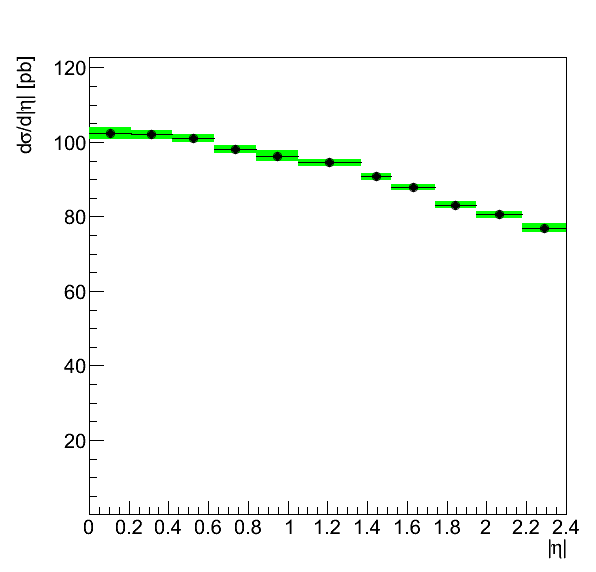
\includegraphics[width=0.27\textwidth]{/home/antonk/SupportingDocument/Wmunu/figures/res/Wmn_UNFABS_2D_PT20_NEG_UnfAbs_2d_Slice_3}
        }
       \subfigure[\ptThree]{%
	  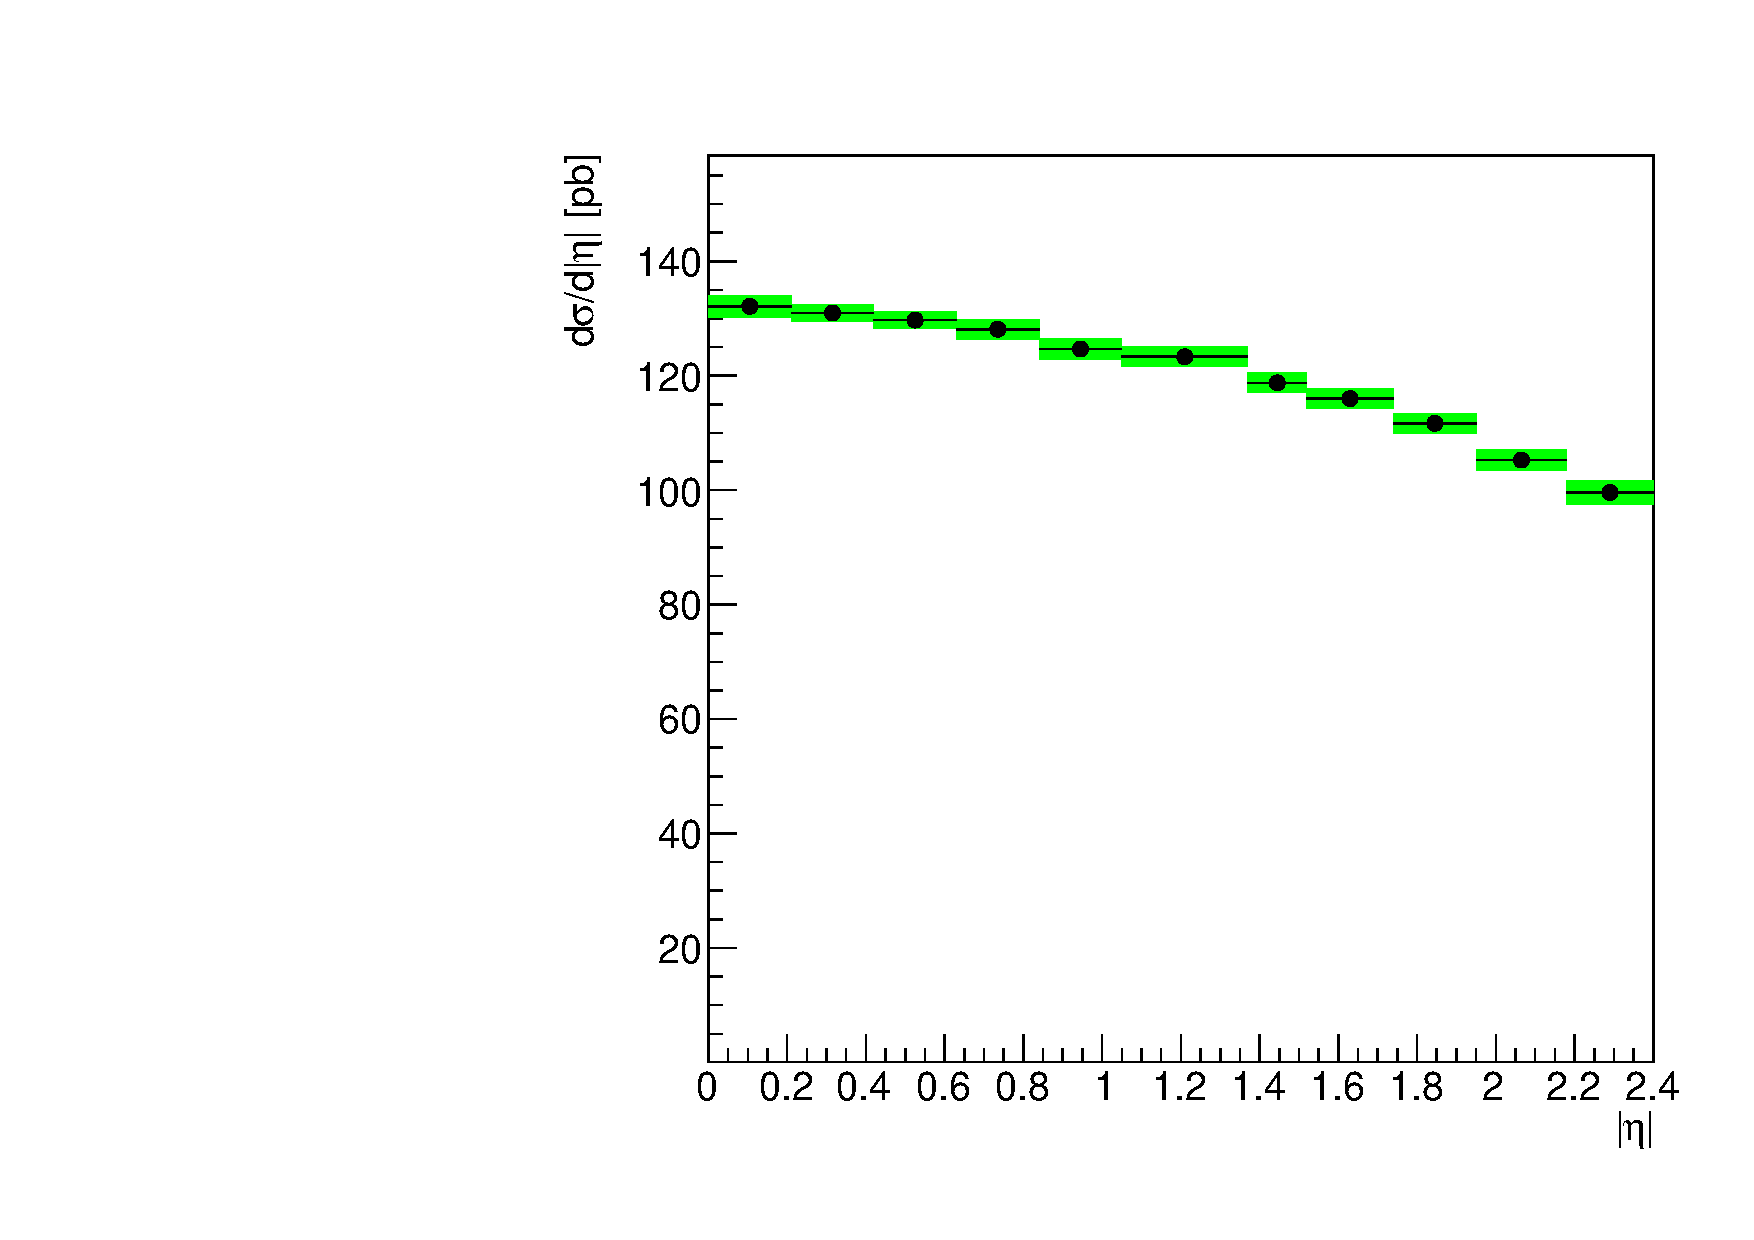
\includegraphics[width=0.27\textwidth]{/home/antonk/SupportingDocument/Wmunu/figures/res/Wmn_UNFABS_2D_PT20_NEG_UnfAbs_2d_Slice_4}
        } \\
       \subfigure[\ptFour]{%
	  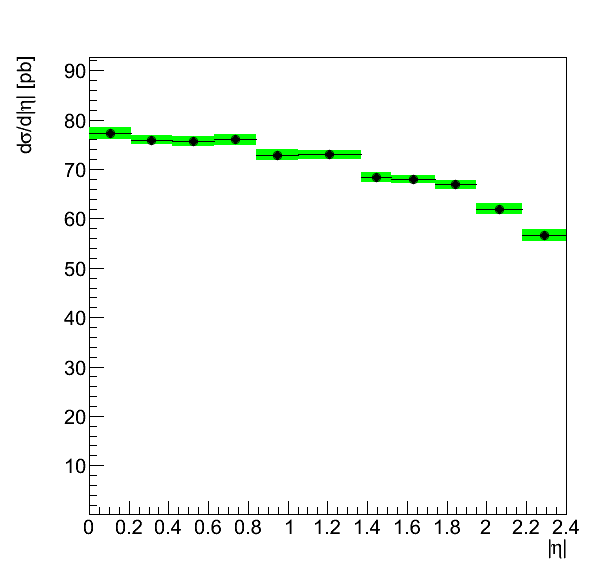
\includegraphics[width=0.27\textwidth]{/home/antonk/SupportingDocument/Wmunu/figures/res/Wmn_UNFABS_2D_PT20_NEG_UnfAbs_2d_Slice_5}
        }
       \subfigure[\ptFive]{%
	  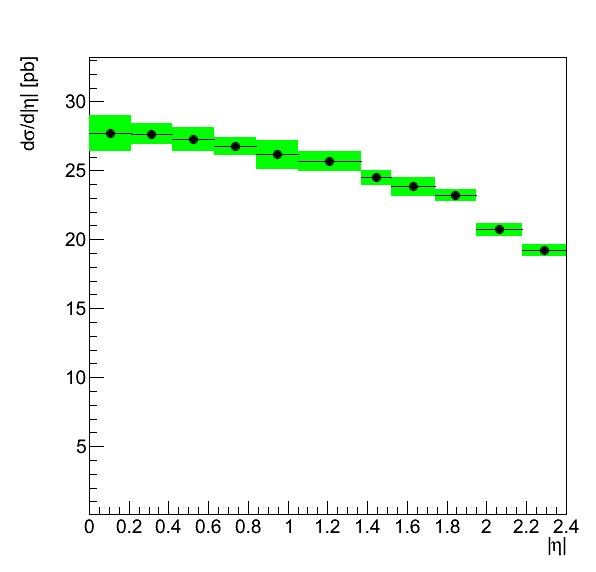
\includegraphics[width=0.27\textwidth]{/home/antonk/SupportingDocument/Wmunu/figures/res/Wmn_UNFABS_2D_PT20_NEG_UnfAbs_2d_Slice_6}
        }
       \subfigure[\ptSix]{%
	  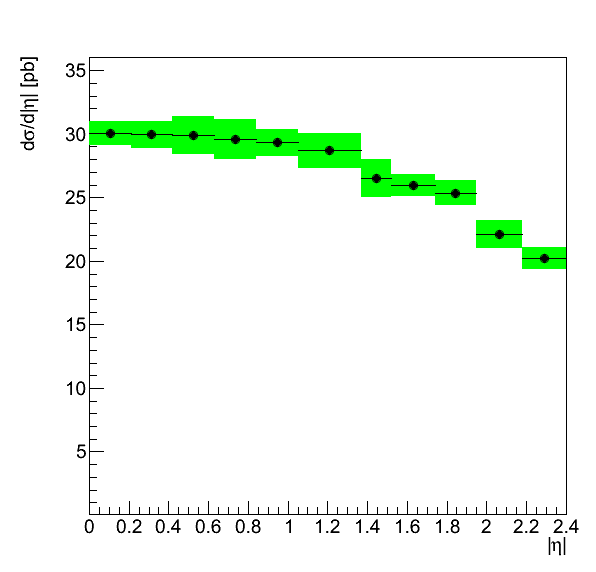
\includegraphics[width=0.27\textwidth]{/home/antonk/SupportingDocument/Wmunu/figures/res/Wmn_UNFABS_2D_PT20_NEG_UnfAbs_2d_Slice_7}
       } 
 \end{center}
\end{figure}
}

%%%%%%% Back-up slides %%%%%%%%%%
\appendix
\newcounter{finalframe}
\setcounter{finalframe}{\value{framenumber}}

\slide{}
{
\centering
\Huge Back-up slides
}

\slide{ Double-differential uncertainties }
{
Effect of latest updates on double-differential uncertainties. \\
Summary: appreciable change in the first and last $p_T$ bins; small elsewhere.
}

\slide{ $20 < p_T < 25$ }
{
\colb[T]
\column{.5\textwidth}
\centering
\only<1>{ \small{ $W^{-}$: CombinationInputs v8} }
\only<2>{ \small{ $W^{-}$: CombinationInputs vX} }
\includegraphics[width=1.0\textwidth]<1>{dates/20130418/figures/v21/Wmn_SYSTEM30_2D_PT20_NEG_Unc_2d_Slice_1}
\includegraphics[width=1.0\textwidth]<2>{dates/20130418/figures/v23/Wmn_SYSTEM30_2D_PT20_NEG_Unc_2d_Slice_1}
\column{.5\textwidth}

\centering
\only<1>{ \small{ $W^{+}$: CombinationInputs v8} }
\only<2>{ \small{ $W^{+}$: CombinationInputs vX} }
\includegraphics[width=1.0\textwidth]<1>{dates/20130418/figures/v21/Wmn_SYSTEM30_2D_PT20_POS_Unc_2d_Slice_1}
\includegraphics[width=1.0\textwidth]<2>{dates/20130418/figures/v23/Wmn_SYSTEM30_2D_PT20_POS_Unc_2d_Slice_1}
\cole
}

\slide{ $25 < p_T < 30$ }
{
\colb[T]
\column{.5\textwidth}
\centering
\only<1>{ \small{ $W^{-}$: CombinationInputs v8} }
\only<2>{ \small{ $W^{-}$: CombinationInputs vX} }
\includegraphics[width=1.0\textwidth]<1>{dates/20130418/figures/v21/Wmn_SYSTEM_2D_PT20_NEG_Unc_2d_Slice_2}
\includegraphics[width=1.0\textwidth]<2>{dates/20130418/figures/v23/Wmn_SYSTEM_2D_PT20_NEG_Unc_2d_Slice_2}
\column{.5\textwidth}

\centering
\only<1>{ \small{ $W^{+}$: CombinationInputs v8} }
\only<2>{ \small{ $W^{+}$: CombinationInputs vX} }
\includegraphics[width=1.0\textwidth]<1>{dates/20130418/figures/v21/Wmn_SYSTEM_2D_PT20_POS_Unc_2d_Slice_2}
\includegraphics[width=1.0\textwidth]<2>{dates/20130418/figures/v23/Wmn_SYSTEM_2D_PT20_POS_Unc_2d_Slice_2}
\cole
}

\slide{ $30 < p_T < 35$ }
{
\colb[T]
\column{.5\textwidth}
\centering
\only<1>{ \small{ $W^{-}$: CombinationInputs v8} }
\only<2>{ \small{ $W^{-}$: CombinationInputs vX} }
\includegraphics[width=1.0\textwidth]<1>{dates/20130418/figures/v21/Wmn_SYSTEM_2D_PT20_NEG_Unc_2d_Slice_3}
\includegraphics[width=1.0\textwidth]<2>{dates/20130418/figures/v23/Wmn_SYSTEM_2D_PT20_NEG_Unc_2d_Slice_3}
\column{.5\textwidth}

\centering
\only<1>{ \small{ $W^{+}$: CombinationInputs v8} }
\only<2>{ \small{ $W^{+}$: CombinationInputs vX} }
\includegraphics[width=1.0\textwidth]<1>{dates/20130418/figures/v21/Wmn_SYSTEM_2D_PT20_POS_Unc_2d_Slice_3}
\includegraphics[width=1.0\textwidth]<2>{dates/20130418/figures/v23/Wmn_SYSTEM_2D_PT20_POS_Unc_2d_Slice_3}
\cole
}

\slide{ $35 < p_T < 40$ }
{
\colb[T]
\column{.5\textwidth}
\centering
\only<1>{ \small{ $W^{-}$: CombinationInputs v8} }
\only<2>{ \small{ $W^{-}$: CombinationInputs vX} }
\includegraphics[width=1.0\textwidth]<1>{dates/20130418/figures/v21/Wmn_SYSTEM_2D_PT20_NEG_Unc_2d_Slice_4}
\includegraphics[width=1.0\textwidth]<2>{dates/20130418/figures/v23/Wmn_SYSTEM_2D_PT20_NEG_Unc_2d_Slice_4}
\column{.5\textwidth}

\centering
\only<1>{ \small{ $W^{+}$: CombinationInputs v8} }
\only<2>{ \small{ $W^{+}$: CombinationInputs vX} }
\includegraphics[width=1.0\textwidth]<1>{dates/20130418/figures/v21/Wmn_SYSTEM_2D_PT20_POS_Unc_2d_Slice_4}
\includegraphics[width=1.0\textwidth]<2>{dates/20130418/figures/v23/Wmn_SYSTEM_2D_PT20_POS_Unc_2d_Slice_4}
\cole
}

\slide{ $40 < p_T < 45$ }
{
\colb[T]
\column{.5\textwidth}
\centering
\only<1>{ \small{ $W^{-}$: CombinationInputs v8} }
\only<2>{ \small{ $W^{-}$: CombinationInputs vX} }
\includegraphics[width=1.0\textwidth]<1>{dates/20130418/figures/v21/Wmn_SYSTEM_2D_PT20_NEG_Unc_2d_Slice_5}
\includegraphics[width=1.0\textwidth]<2>{dates/20130418/figures/v23/Wmn_SYSTEM_2D_PT20_NEG_Unc_2d_Slice_5}
\column{.5\textwidth}

\centering
\only<1>{ \small{ $W^{+}$: CombinationInputs v8} }
\only<2>{ \small{ $W^{+}$: CombinationInputs vX} }
\includegraphics[width=1.0\textwidth]<1>{dates/20130418/figures/v21/Wmn_SYSTEM_2D_PT20_POS_Unc_2d_Slice_5}
\includegraphics[width=1.0\textwidth]<2>{dates/20130418/figures/v23/Wmn_SYSTEM_2D_PT20_POS_Unc_2d_Slice_5}
\cole
}

\slide{ $45 < p_T < 50$ }
{
\colb[T]
\column{.5\textwidth}
\centering
\only<1>{ \small{ $W^{-}$: CombinationInputs v8} }
\only<2>{ \small{ $W^{-}$: CombinationInputs vX} }
\includegraphics[width=1.0\textwidth]<1>{dates/20130418/figures/v21/Wmn_SYSTEM_2D_PT20_NEG_Unc_2d_Slice_6}
\includegraphics[width=1.0\textwidth]<2>{dates/20130418/figures/v23/Wmn_SYSTEM_2D_PT20_NEG_Unc_2d_Slice_6}
\column{.5\textwidth}

\centering
\only<1>{ \small{ $W^{+}$: CombinationInputs v8} }
\only<2>{ \small{ $W^{+}$: CombinationInputs vX} }
\includegraphics[width=1.0\textwidth]<1>{dates/20130418/figures/v21/Wmn_SYSTEM_2D_PT20_POS_Unc_2d_Slice_6}
\includegraphics[width=1.0\textwidth]<2>{dates/20130418/figures/v23/Wmn_SYSTEM_2D_PT20_POS_Unc_2d_Slice_6}
\cole
}

\slide{ $p_T > 50$ }
{
\colb[T]
\column{.5\textwidth}
\centering
\only<1>{ \small{ $W^{-}$: CombinationInputs v8} }
\only<2>{ \small{ $W^{-}$: CombinationInputs vX} }
\includegraphics[width=1.0\textwidth]<1>{dates/20130418/figures/v21/Wmn_SYSTEM_2D_PT20_NEG_Unc_2d_Slice_7}
\includegraphics[width=1.0\textwidth]<2>{dates/20130418/figures/v23/Wmn_SYSTEM_2D_PT20_NEG_Unc_2d_Slice_7}
\column{.5\textwidth}

\centering
\only<1>{ \small{ $W^{+}$: CombinationInputs v8} }
\only<2>{ \small{ $W^{+}$: CombinationInputs vX} }
\includegraphics[width=1.0\textwidth]<1>{dates/20130418/figures/v21/Wmn_SYSTEM_2D_PT20_POS_Unc_2d_Slice_7}
\includegraphics[width=1.0\textwidth]<2>{dates/20130418/figures/v23/Wmn_SYSTEM_2D_PT20_POS_Unc_2d_Slice_7}
\cole
}
